%-----------------------------------------------------------------------------%
% LAMPIRAN
%-----------------------------------------------------------------------------%
\newpage
\appendix
\renewcommand{\thetable}{A\arabic{table}}
\renewcommand{\thefigure}{A\arabic{figure}}
\renewcommand{\thelstlisting}{A\arabic{lstlisting}}


\appendices{Surat Pengantar PRO-STEP 01}
\begin{center}
    \frame{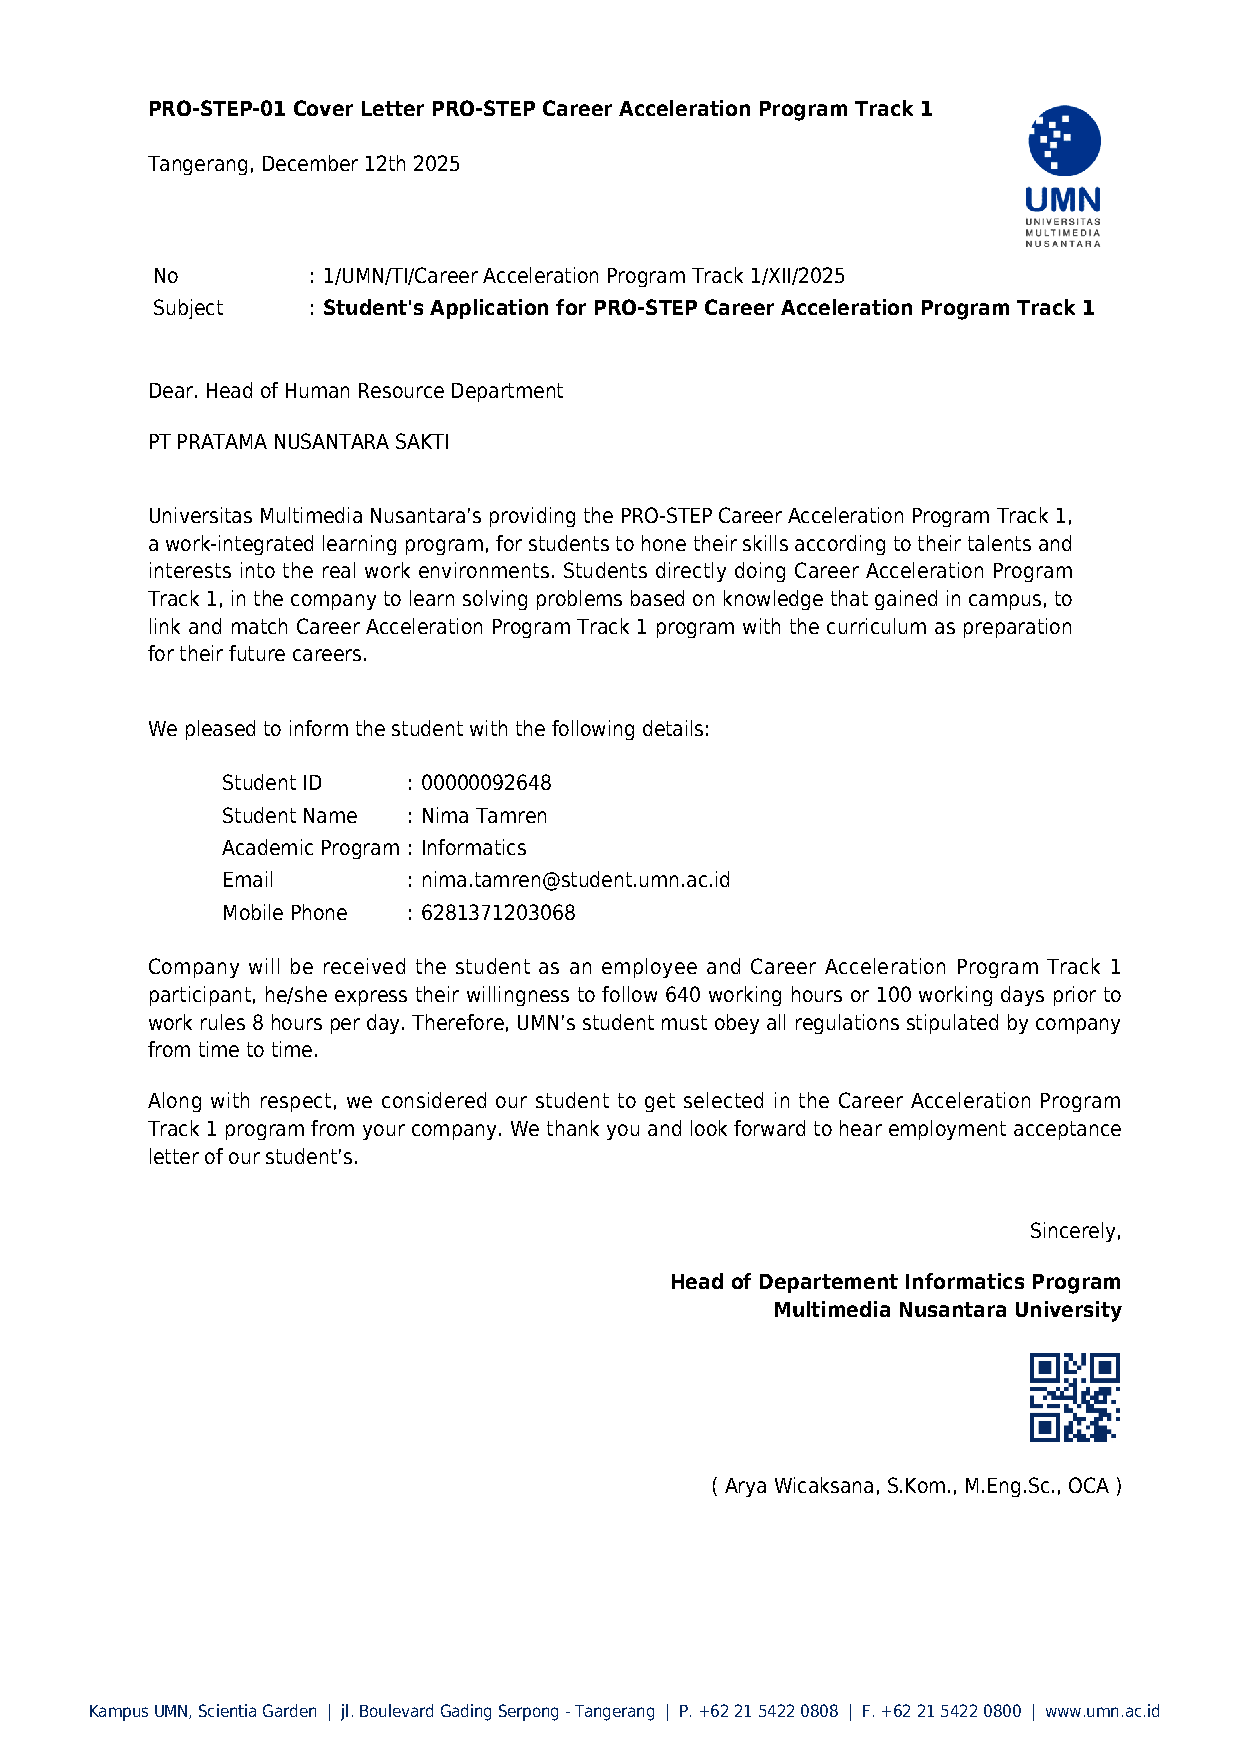
\includegraphics[width=\textwidth,page=1]{assets/pdf/MBKM1_your_name.pdf}}
\end{center}
\clearpage


\appendices{Kartu PRO-STEP 02}
\begin{center}
    \frame{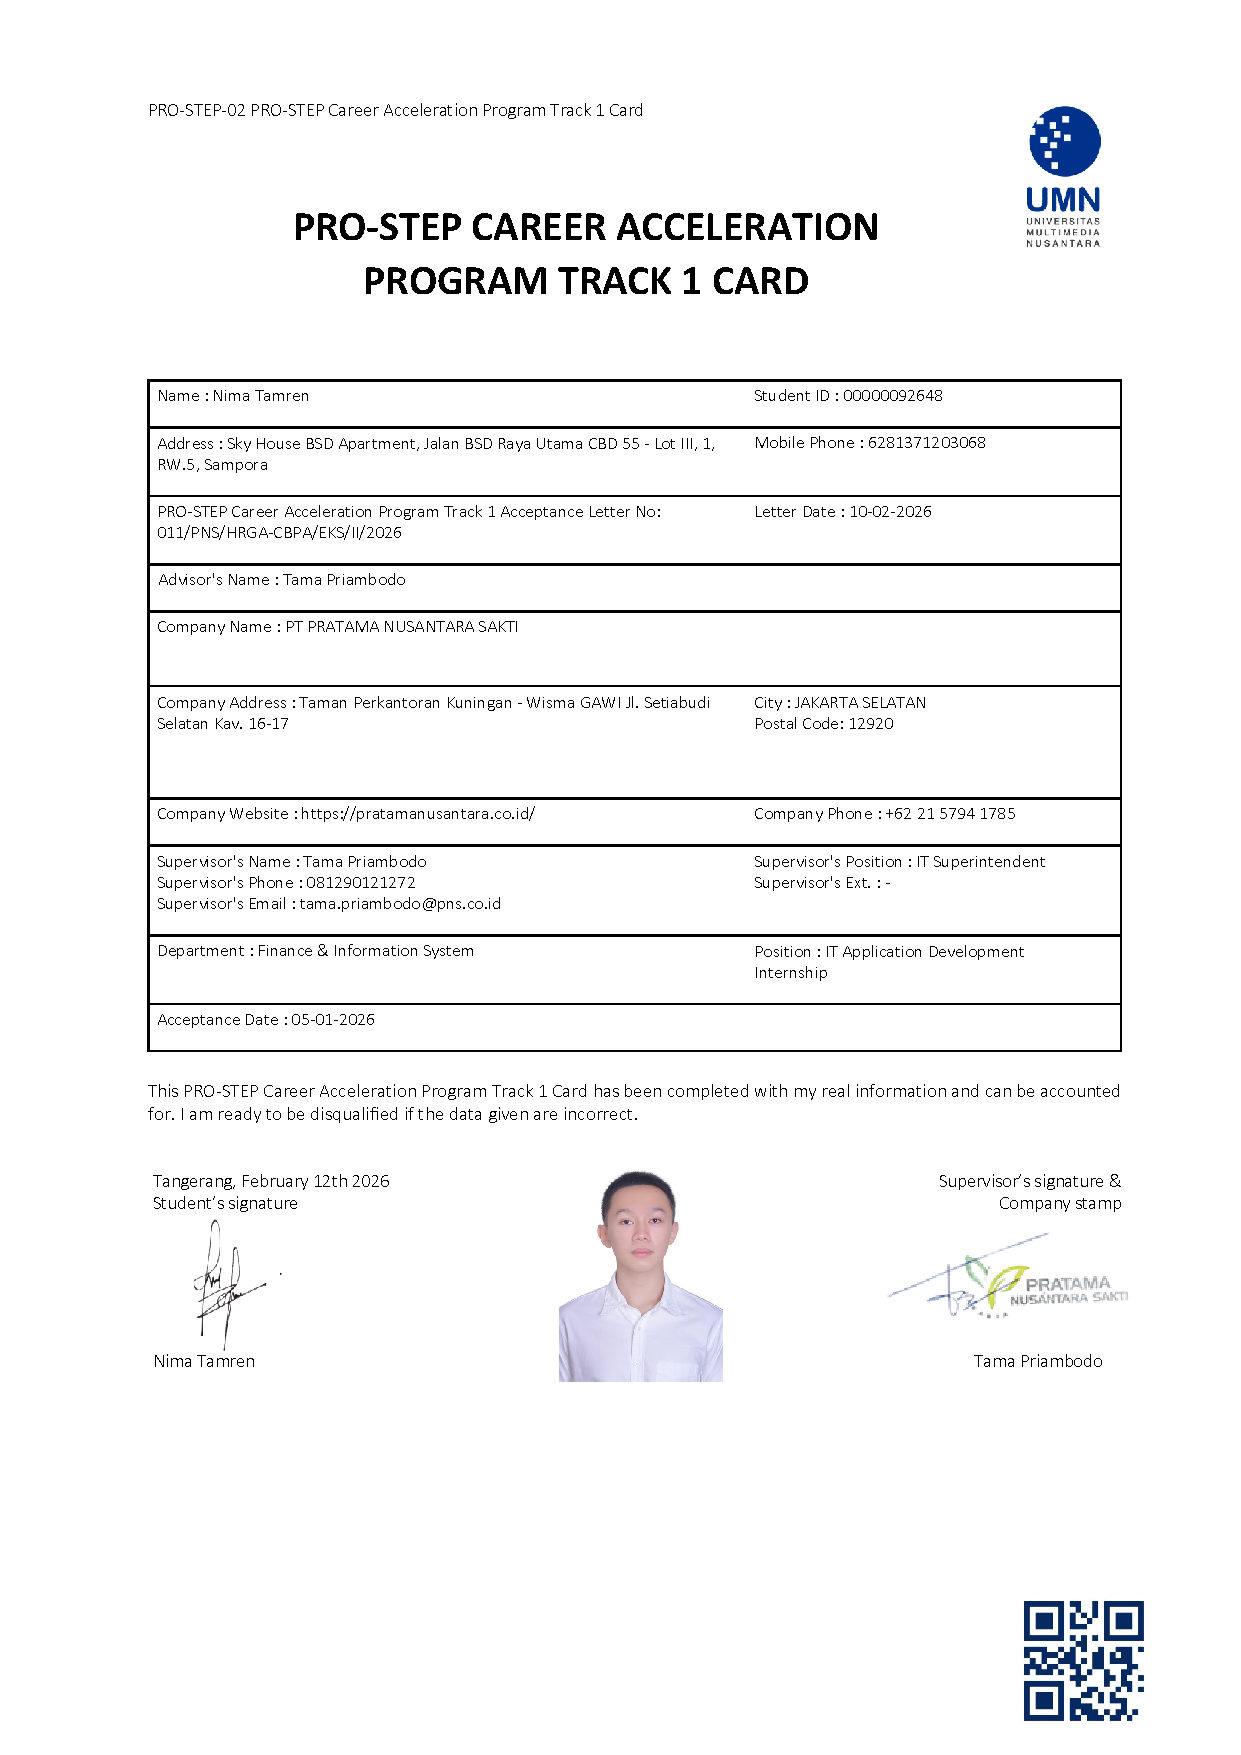
\includegraphics[width=\textwidth,page=1]{assets/pdf/MBKM2_your_name.pdf}}
\end{center}
\clearpage


\appendices{Daily Task PRO-STEP 03}
% Menampilkan SEMUA halaman PDF dengan gaya berbingkai seperti lampiran lain.
\newcount\dtpg \dtpg=1
\loop
    \begin{center}
        \frame{\includegraphics[width=\textwidth,page=\the\dtpg]{assets/pdf/MBKM3_your_name.pdf}}
    \end{center}
    \clearpage
    \advance\dtpg by 1
\ifnum\dtpg<14
\repeat


\appendices{Verifikasi Laporan PRO-STEP 04}
\begin{center}
    \frame{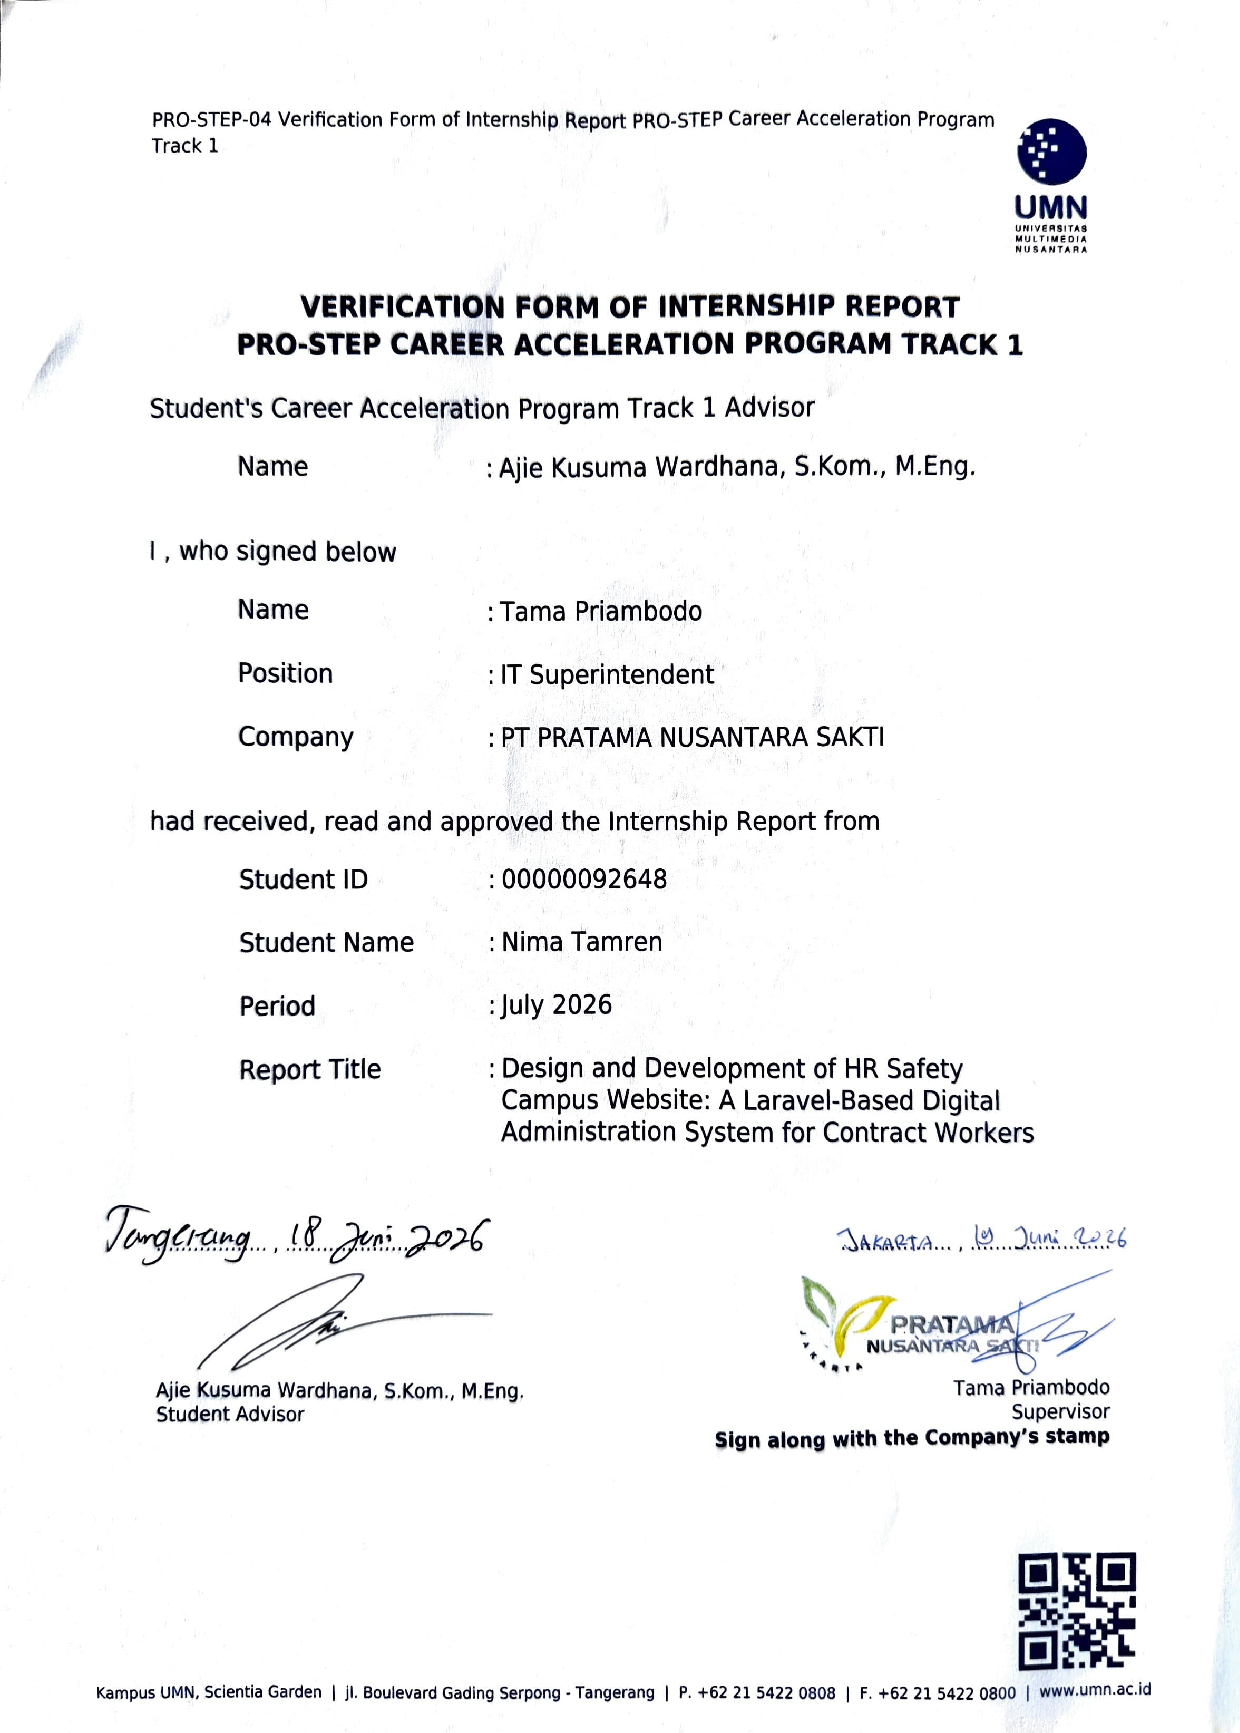
\includegraphics[width=\textwidth,page=1]{assets/pdf/MBKM4_your_name.pdf}}
\end{center}
\clearpage


\appendices{Surat Penerimaan PRO-STEP 05}
\begin{center}
    \frame{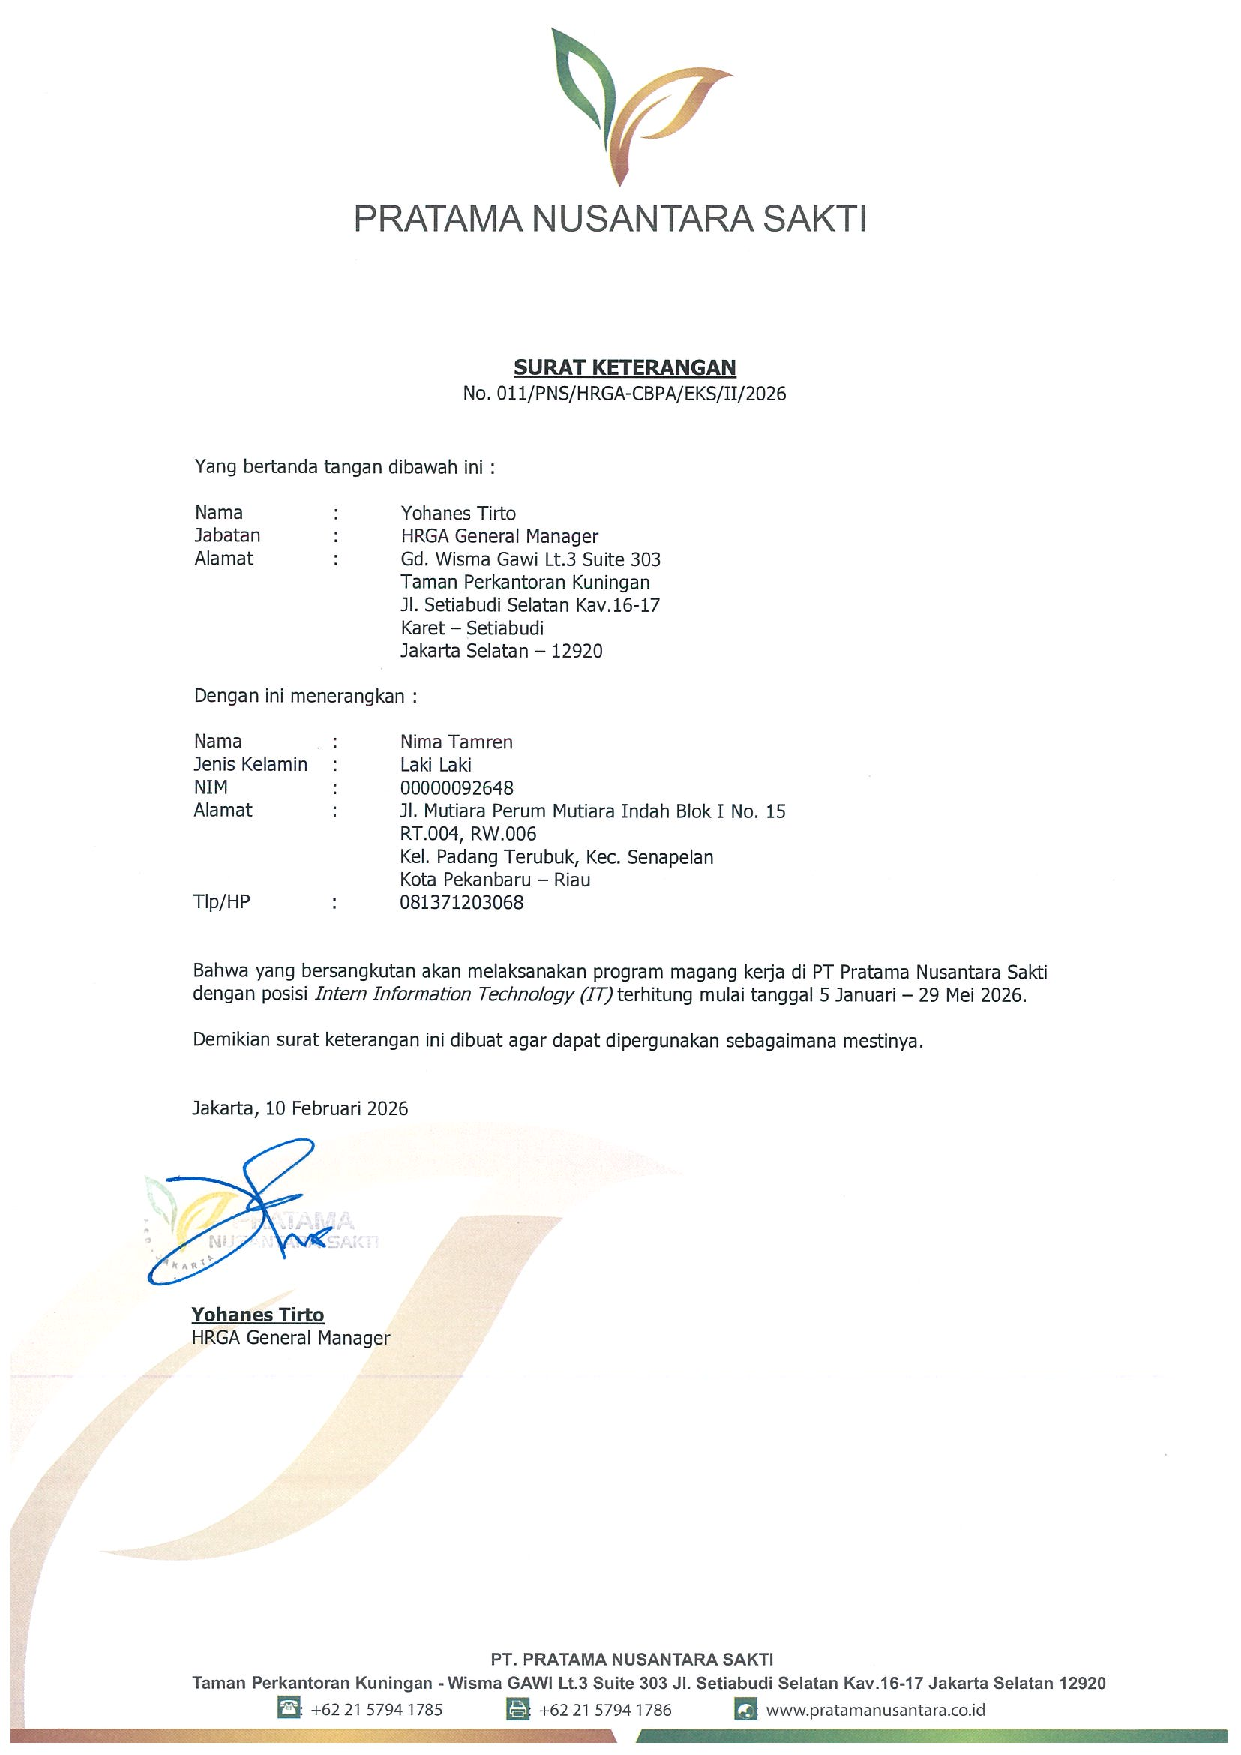
\includegraphics[width=\textwidth,page=1]{assets/pdf/SuratPenerimaan_PROSTEP05.pdf}}
\end{center}
\clearpage


\appendices{Form Bimbingan}
% Form bimbingan terisi (8 kali pertemuan).
\begin{center}
    \frame{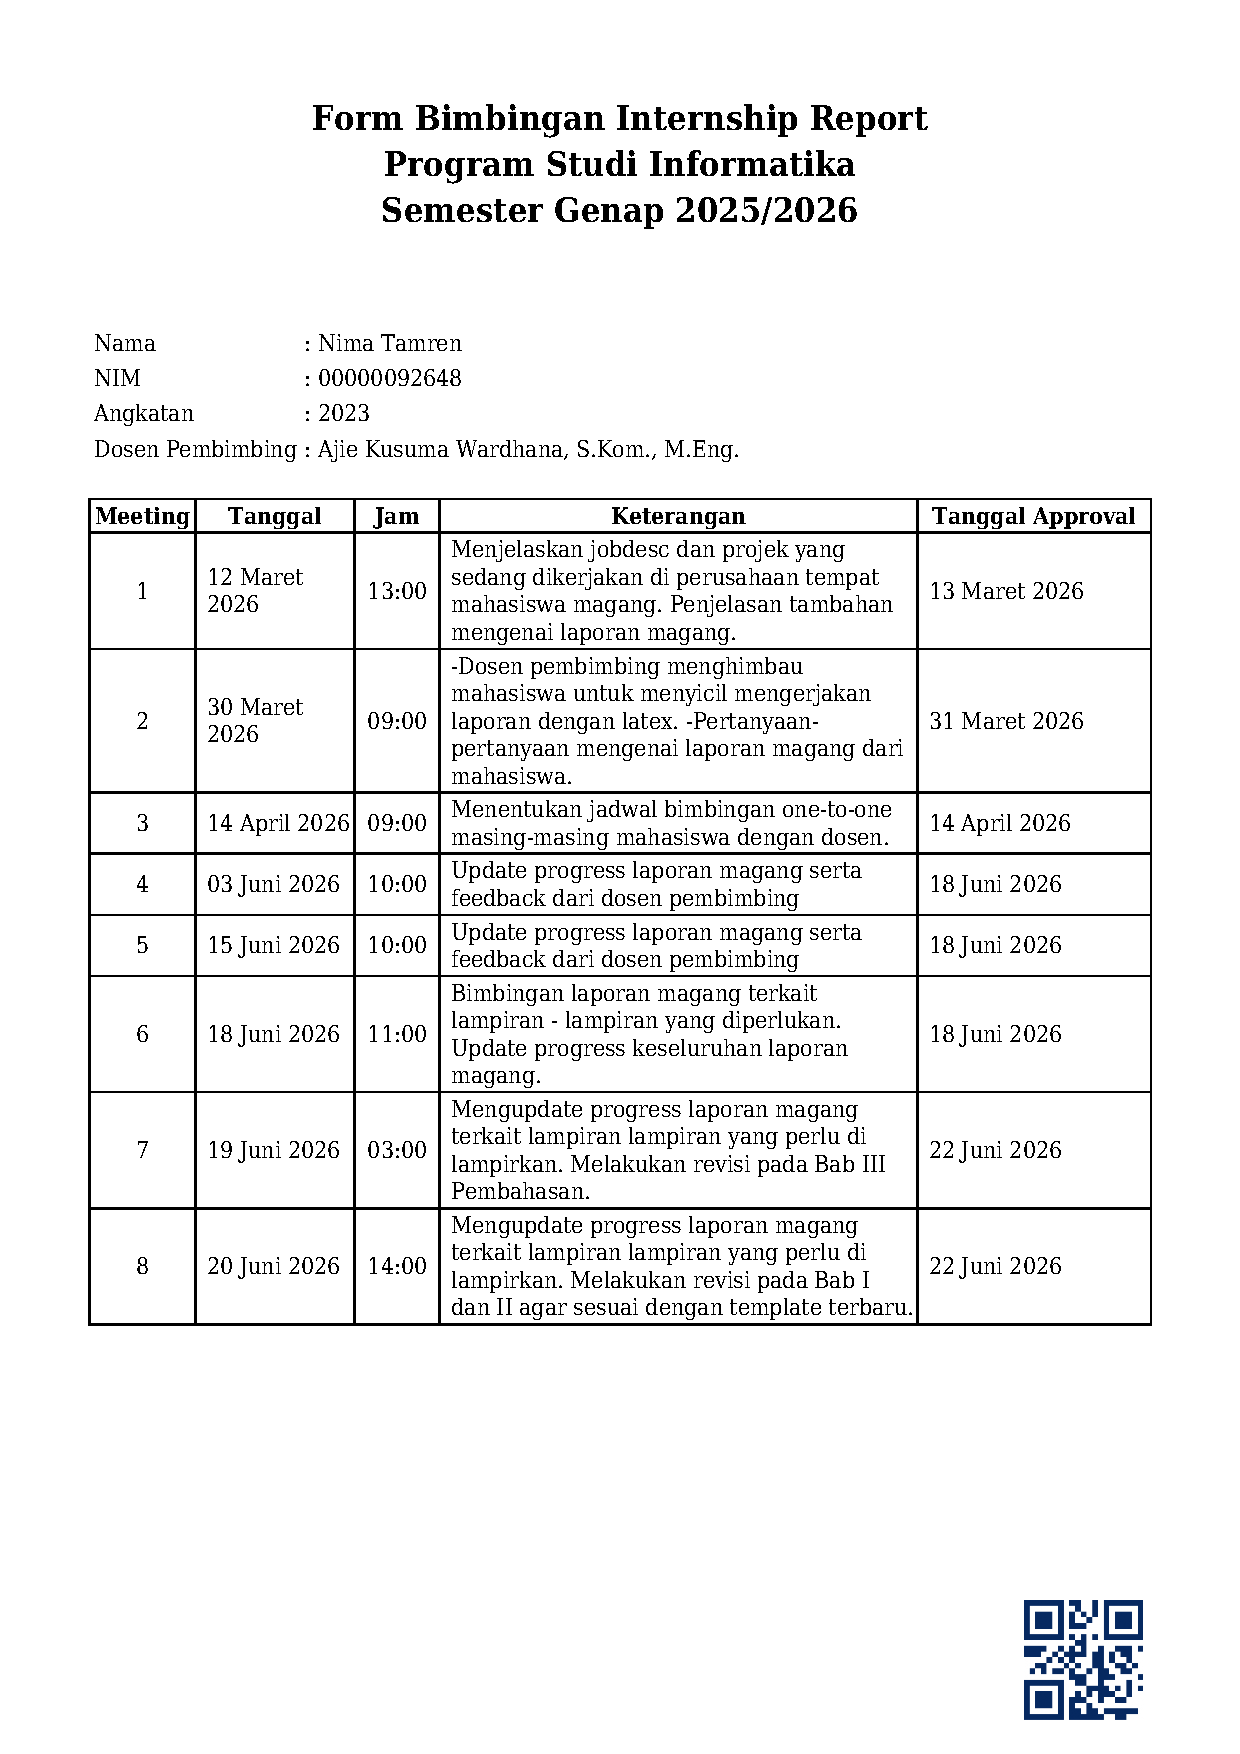
\includegraphics[width=\textwidth,page=1]{assets/pdf/Form_Bimbingan.pdf}}
\end{center}
\clearpage


\appendices{Pengecekan Hasil Similarity Turnitin}
% Tiga halaman pertama hasil pengecekan similarity Turnitin.
\begin{center}
    \frame{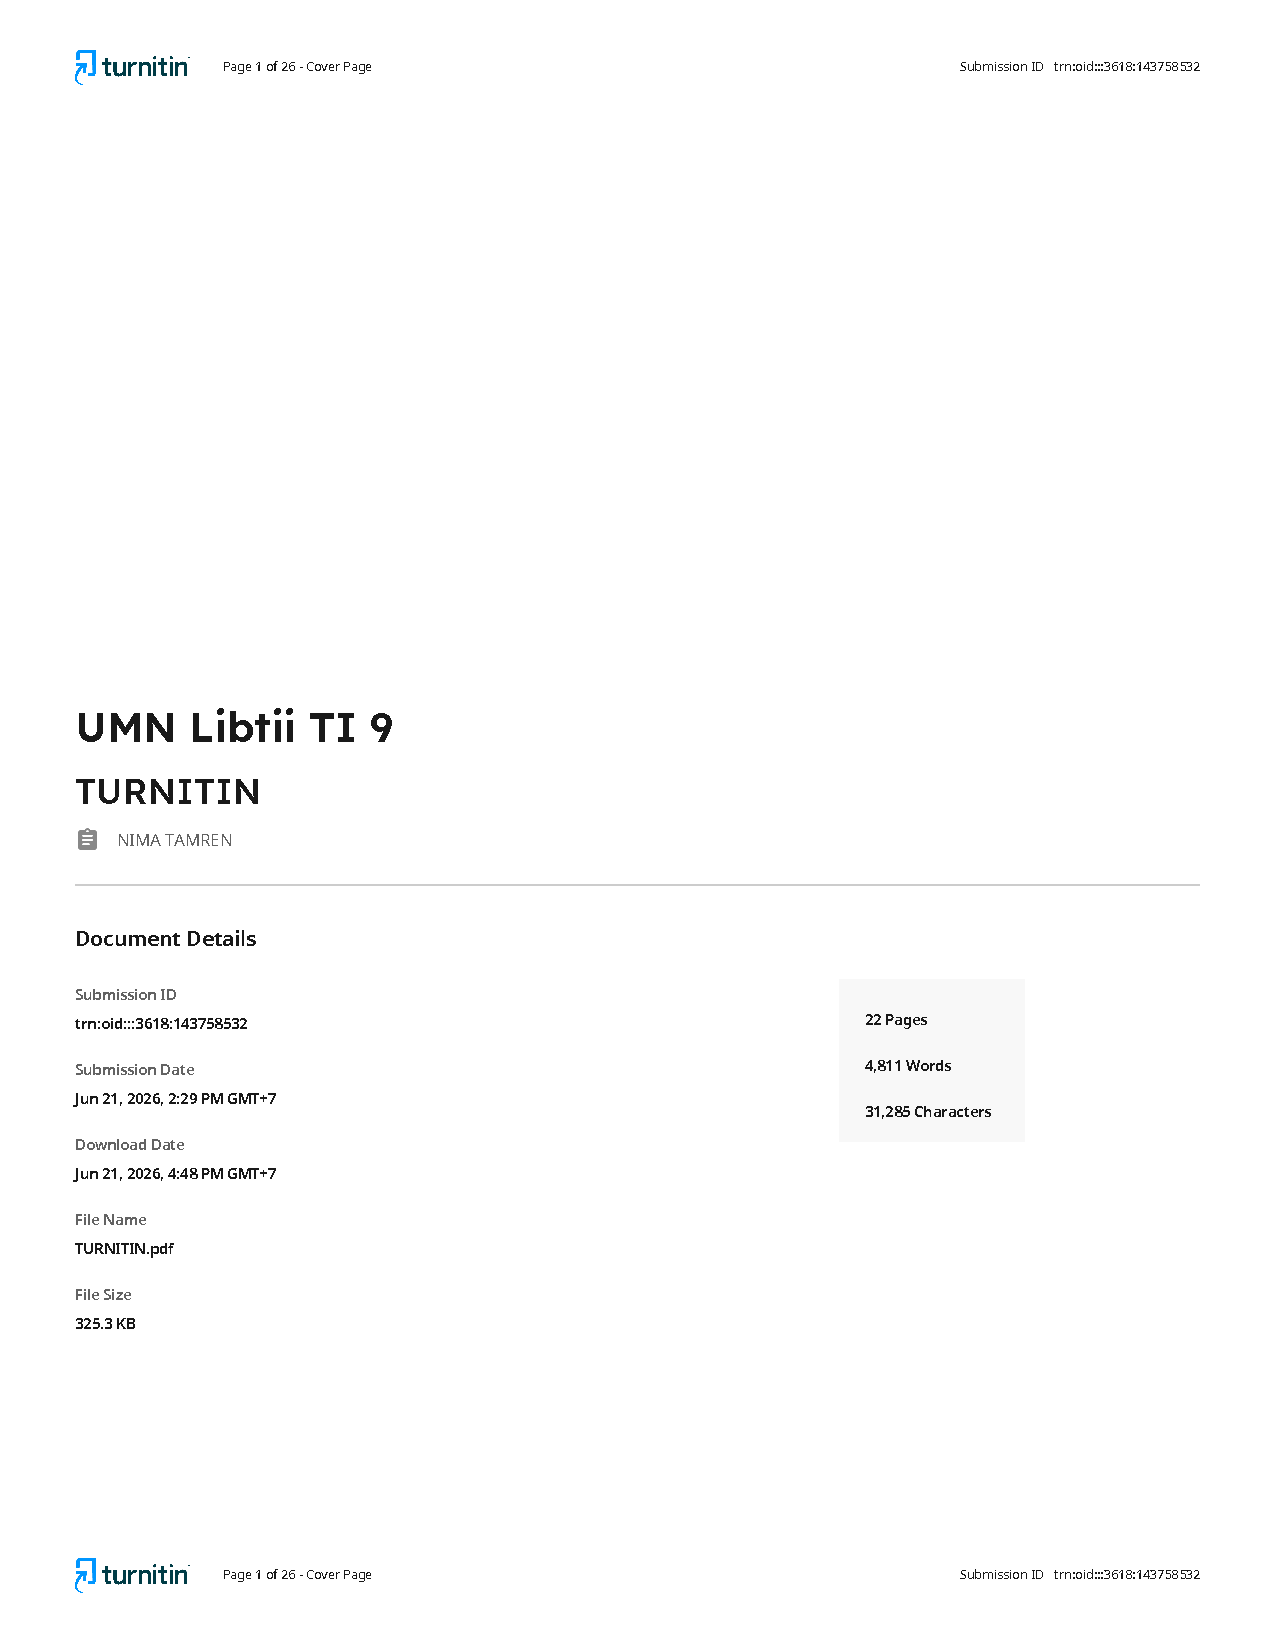
\includegraphics[width=\textwidth,page=1]{assets/pdf/TURNITIN.pdf}}
\end{center}
\clearpage

\begin{center}
    \frame{\includegraphics[width=\textwidth,page=2]{assets/pdf/TURNITIN.pdf}}
\end{center}
\clearpage

\begin{center}
    \frame{\includegraphics[width=\textwidth,page=3]{assets/pdf/TURNITIN.pdf}}
\end{center}
\clearpage


\appendices{Formulir Penggunaan Perangkat Kecerdasan Artifisial (AI)}

\noindent
\begin{tabular}{lcp{9.25cm}}
   Nama Lengkap &:& \penulis \\
   NIM           &:& \nim \\
   Email        &:& nima.tamren@student.umn.ac.id \\
   Program Studi &:& \program \\
   Judul         &:& \judul \\
\end{tabular}

\vspace{\baselineskip}

\noindent
{\small
\renewcommand{\arraystretch}{1.4}
\setlength{\tabcolsep}{4pt}
\begin{longtable}{|c|p{1.9cm}|p{2.2cm}|p{3.1cm}|p{1.8cm}|p{2.3cm}|}
    \hline
    \textbf{No} & \textbf{Nama Tool} & \textbf{Alamat Web/Url} & \textbf{Prompt} & \textbf{Tanggal Akses} & \textbf{Media Output} \\
    \hline
    \endfirsthead
    \hline
    \textbf{No} & \textbf{Nama Tool} & \textbf{Alamat Web/Url} & \textbf{Prompt} & \textbf{Tanggal Akses} & \textbf{Media Output} \\
    \hline
    \endhead
    \hline
    \endfoot
    \hline
    \endlastfoot
    1 & Google Gemini & \url{https://gemini.google.com} & ``Tolong periksa tata bahasa dan ejaan pada bagian Latar Belakang laporan magang ini agar lebih formal dan sesuai kaidah penulisan ilmiah.'' & \textit{06 April 2026} & Saran perbaikan tata bahasa dan ejaan pada bagian Latar Belakang yang kemudian ditinjau dan disesuaikan kembali oleh penulis. \\
    \hline
    2 & Google Gemini & \url{https://gemini.google.com} & ``Apakah Tabel 3.1 (Detail Pekerjaan yang Dilakukan) sudah cukup jelas mendeskripsikan pekerjaan selama magang, atau adakah susunan tabel yang lebih baik?'' & \textit{12 Mei 2026} & Saran penyempurnaan struktur Tabel 3.1 (penambahan kolom modul/fitur dan output serta penggabungan minggu) yang kemudian disesuaikan oleh penulis. \\
    \hline
    3 & Google Gemini & \url{https://gemini.google.com} & ``Bagaimana pendapatmu tentang Bab 3 yang sedang saya susun? Bagian mana yang dapat saya perjelas atau perbaiki?'' & \textit{08 Juni 2026} & Masukan perbaikan Bab 3 (penyelarasan dengan metode \textit{Waterfall}, elaborasi komunikasi dengan klien dan pembersihan data, serta penambahan rujukan visual ke lampiran) yang kemudian ditinjau dan disesuaikan oleh penulis. \\
    \hline
\end{longtable}
}
\clearpage


%=============================================================================%
% LAMPIRAN TAMBAHAN (di luar daftar wajib template): TANGKAPAN LAYAR ANTARMUKA
% Boleh dipertahankan sebagai bukti hasil kerja, atau dihapus jika tidak diminta.
%=============================================================================%
\appendices{Tangkapan Layar Antarmuka Sistem HR Safety Campus}

Bagian ini menampilkan tangkapan layar (\textit{screenshot}) dari antarmuka
sistem \textit{HR Safety Campus} yang dikembangkan selama pelaksanaan kerja
magang, mencakup halaman utama, keenam fitur utama, beserta dasbor pendukungnya.

% --- HALAMAN UTAMA (MAIN MENU) ---
\begin{figure}[H]
    \centering
    \frame{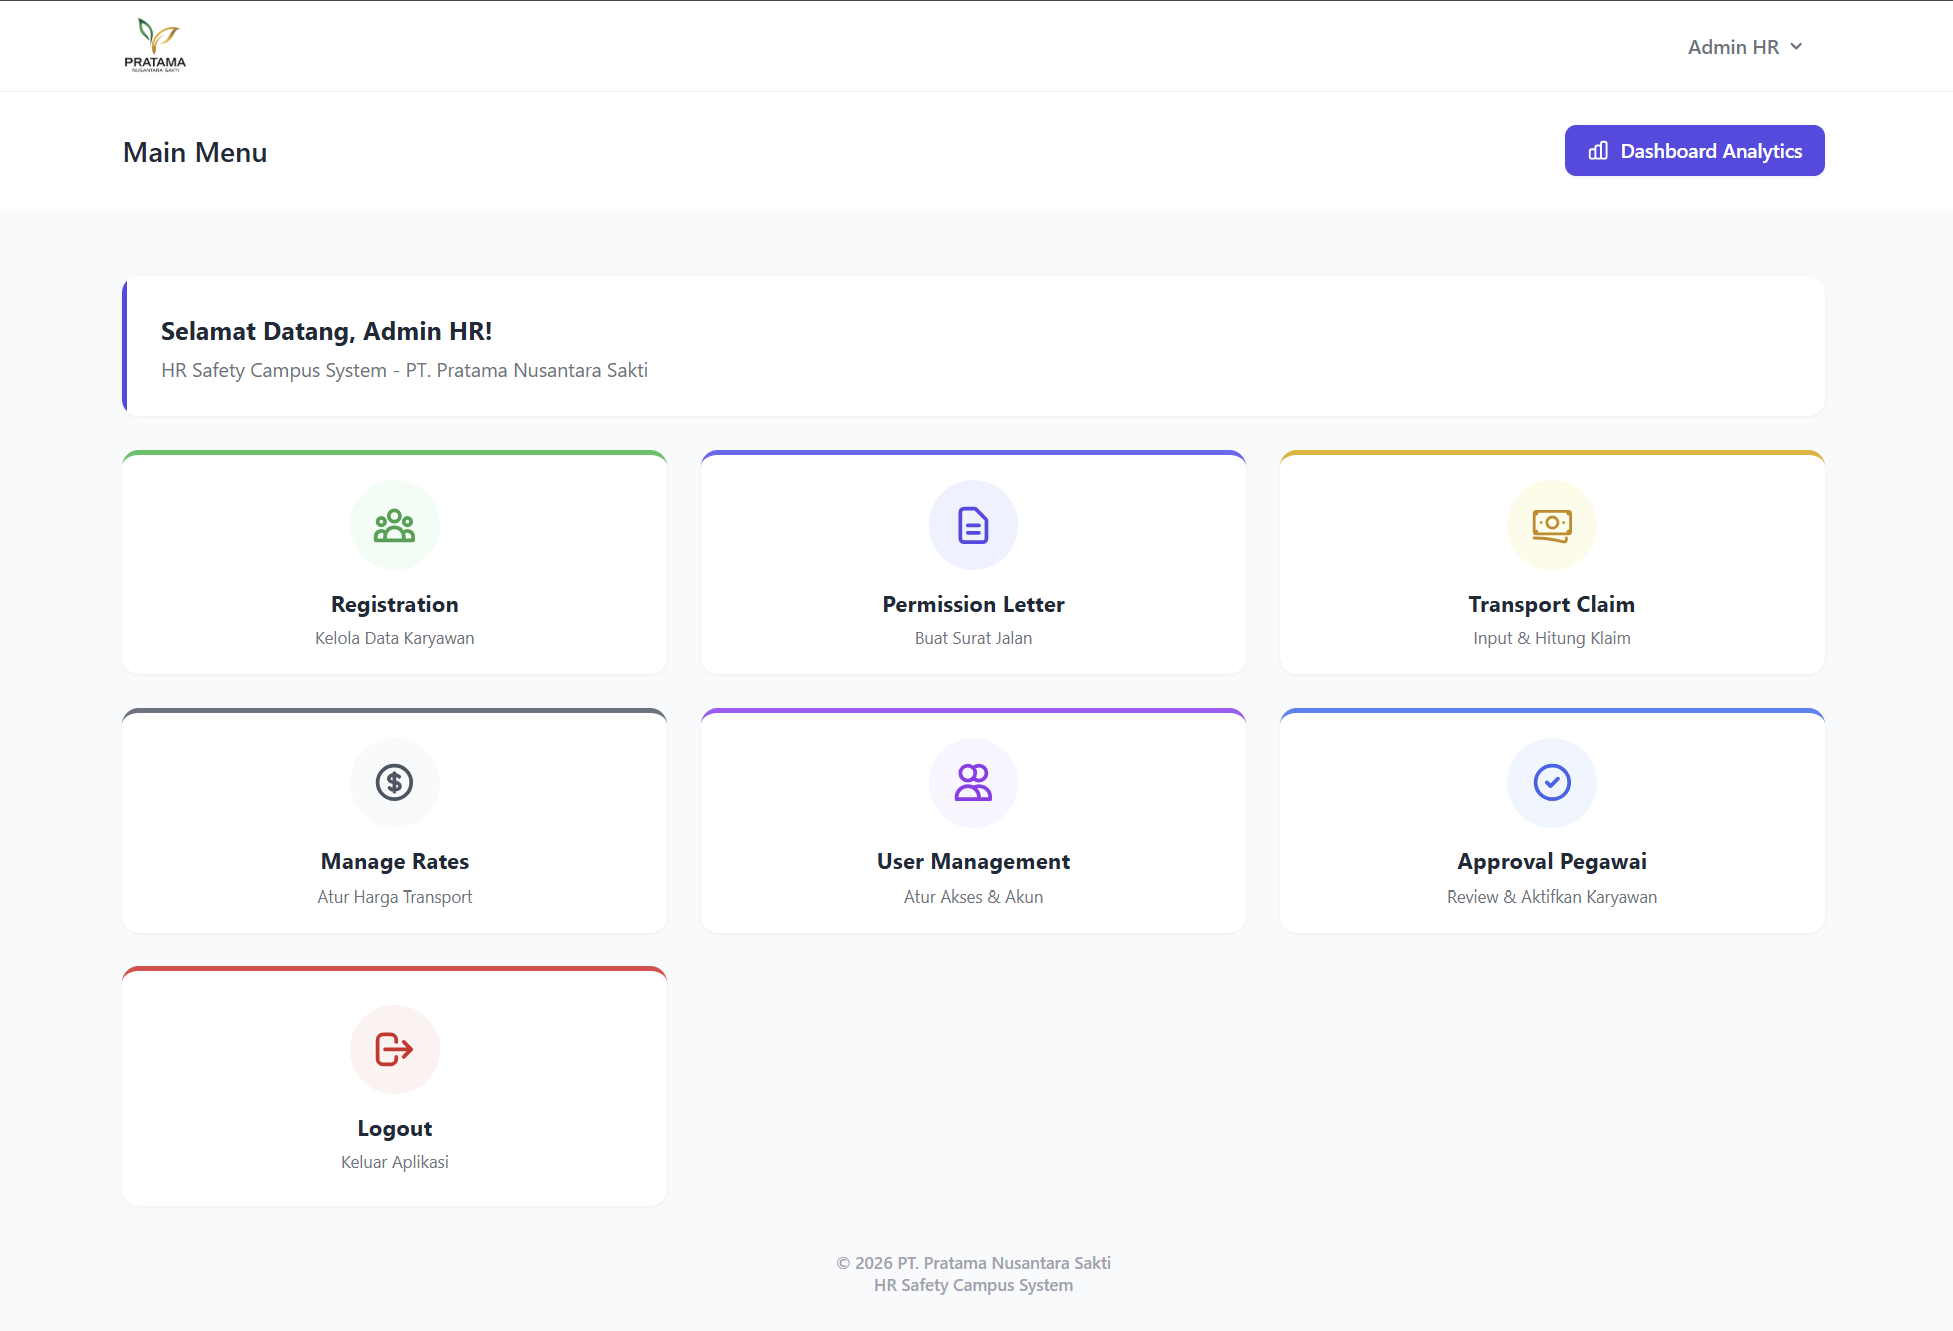
\includegraphics[width=0.9\textwidth]{assets/pics/Main_Menu.png}}
    \caption{Halaman Main Menu sistem HR Safety Campus}
    \label{fig:ui-main-menu}
\end{figure}
\clearpage

% --- FITUR 1: REGISTRASI TENAGA KERJA ---
\begin{figure}[H]
    \centering
    \frame{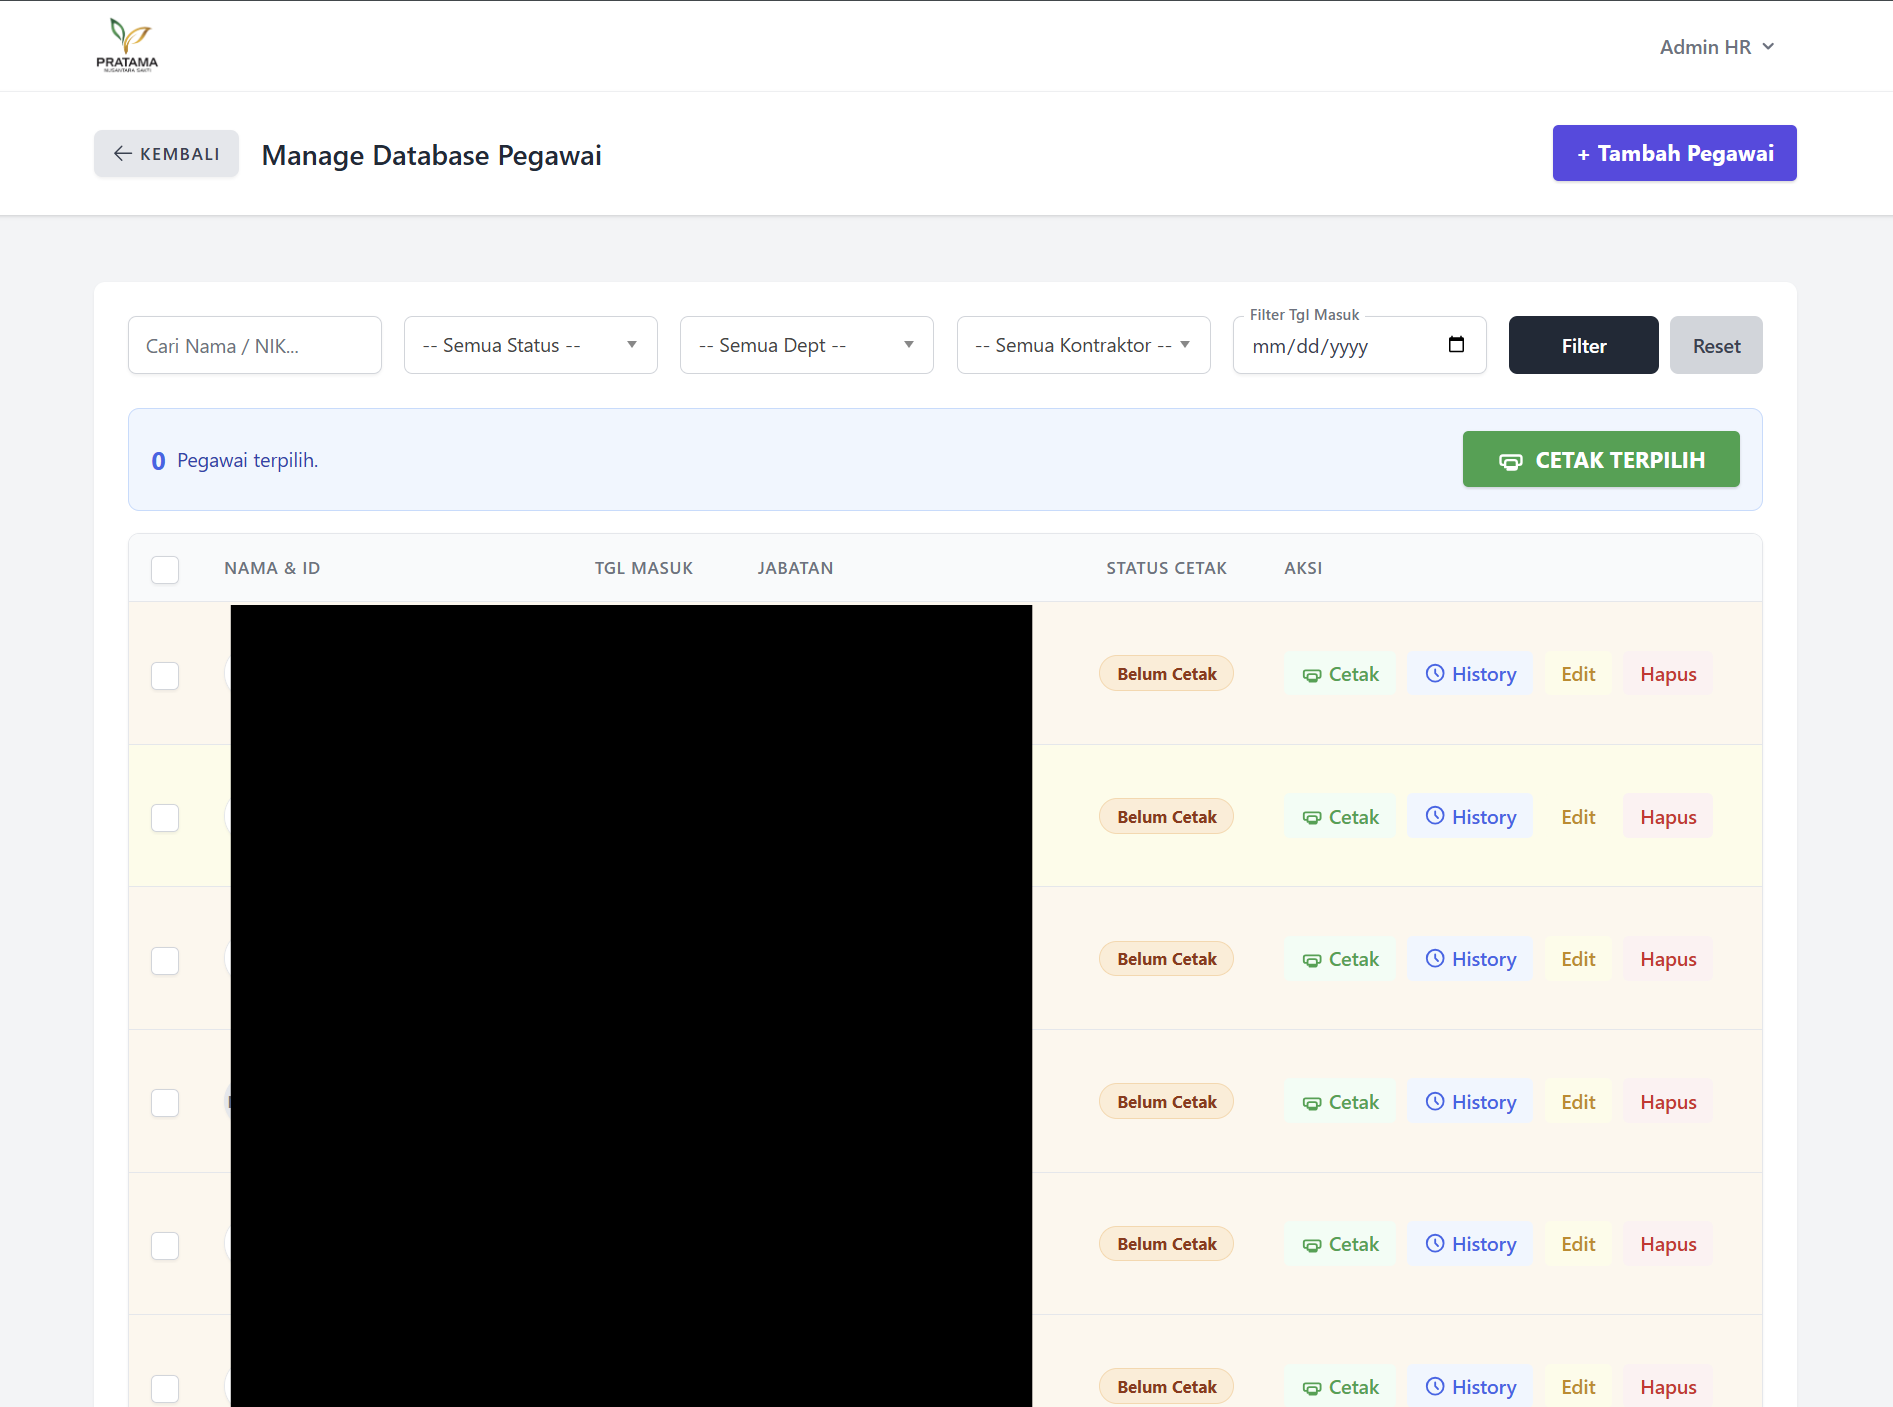
\includegraphics[width=0.9\textwidth]{assets/pics/Main_Menu_UI.png}}
    \caption{Halaman Manage Database Pegawai pada fitur Registrasi Tenaga Kerja}
    \label{fig:ui-manage-pegawai}
\end{figure}

\begin{figure}[H]
    \centering
    \frame{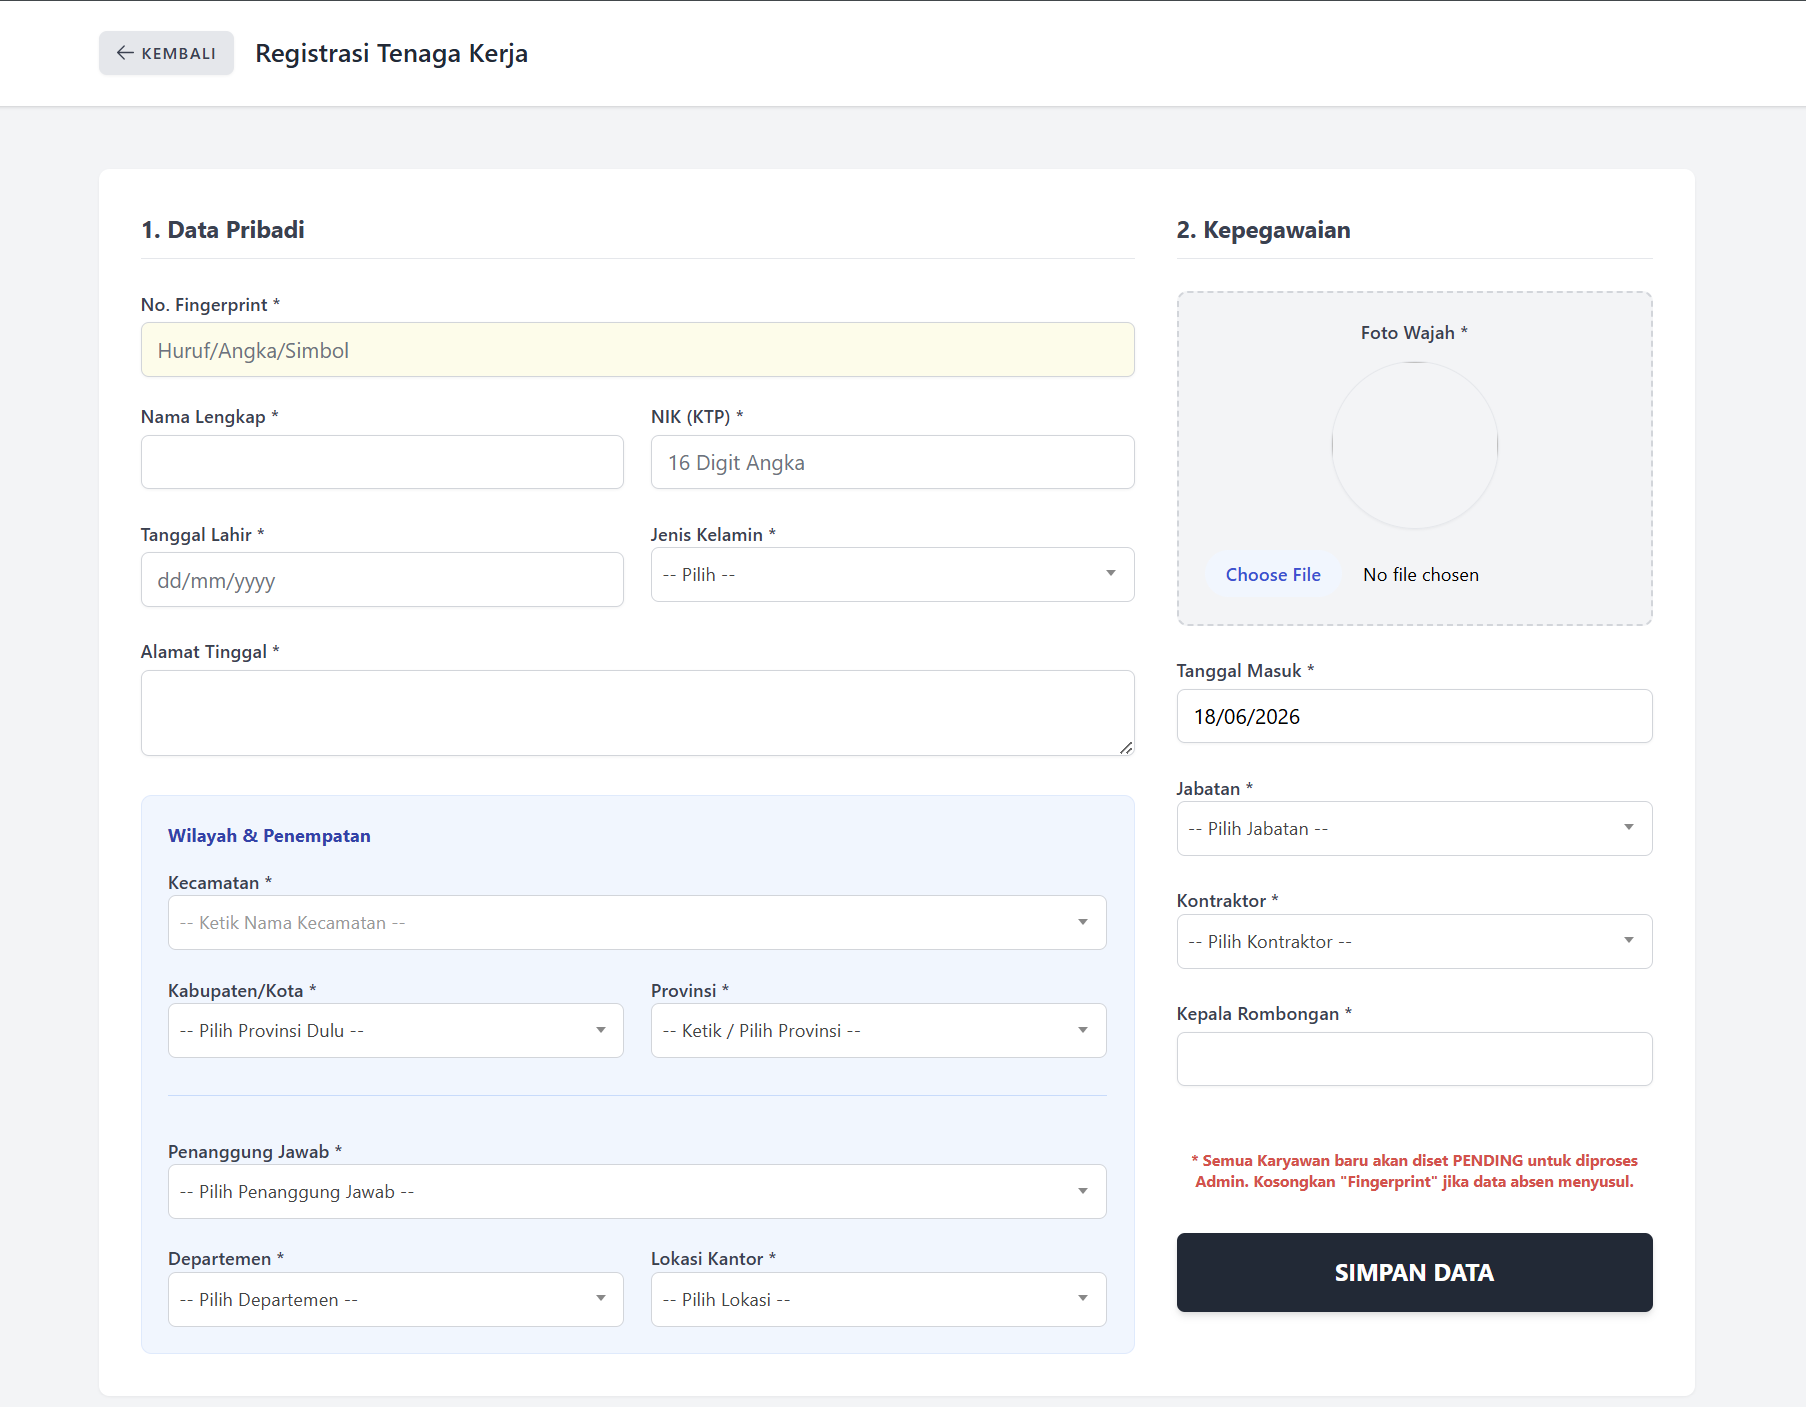
\includegraphics[width=0.9\textwidth]{assets/pics/Registration.png}}
    \caption{Formulir Registrasi Tenaga Kerja baru}
    \label{fig:ui-registrasi}
\end{figure}
\clearpage

% --- FITUR 2: KLAIM TRANSPORT ---
\begin{figure}[H]
    \centering
    \frame{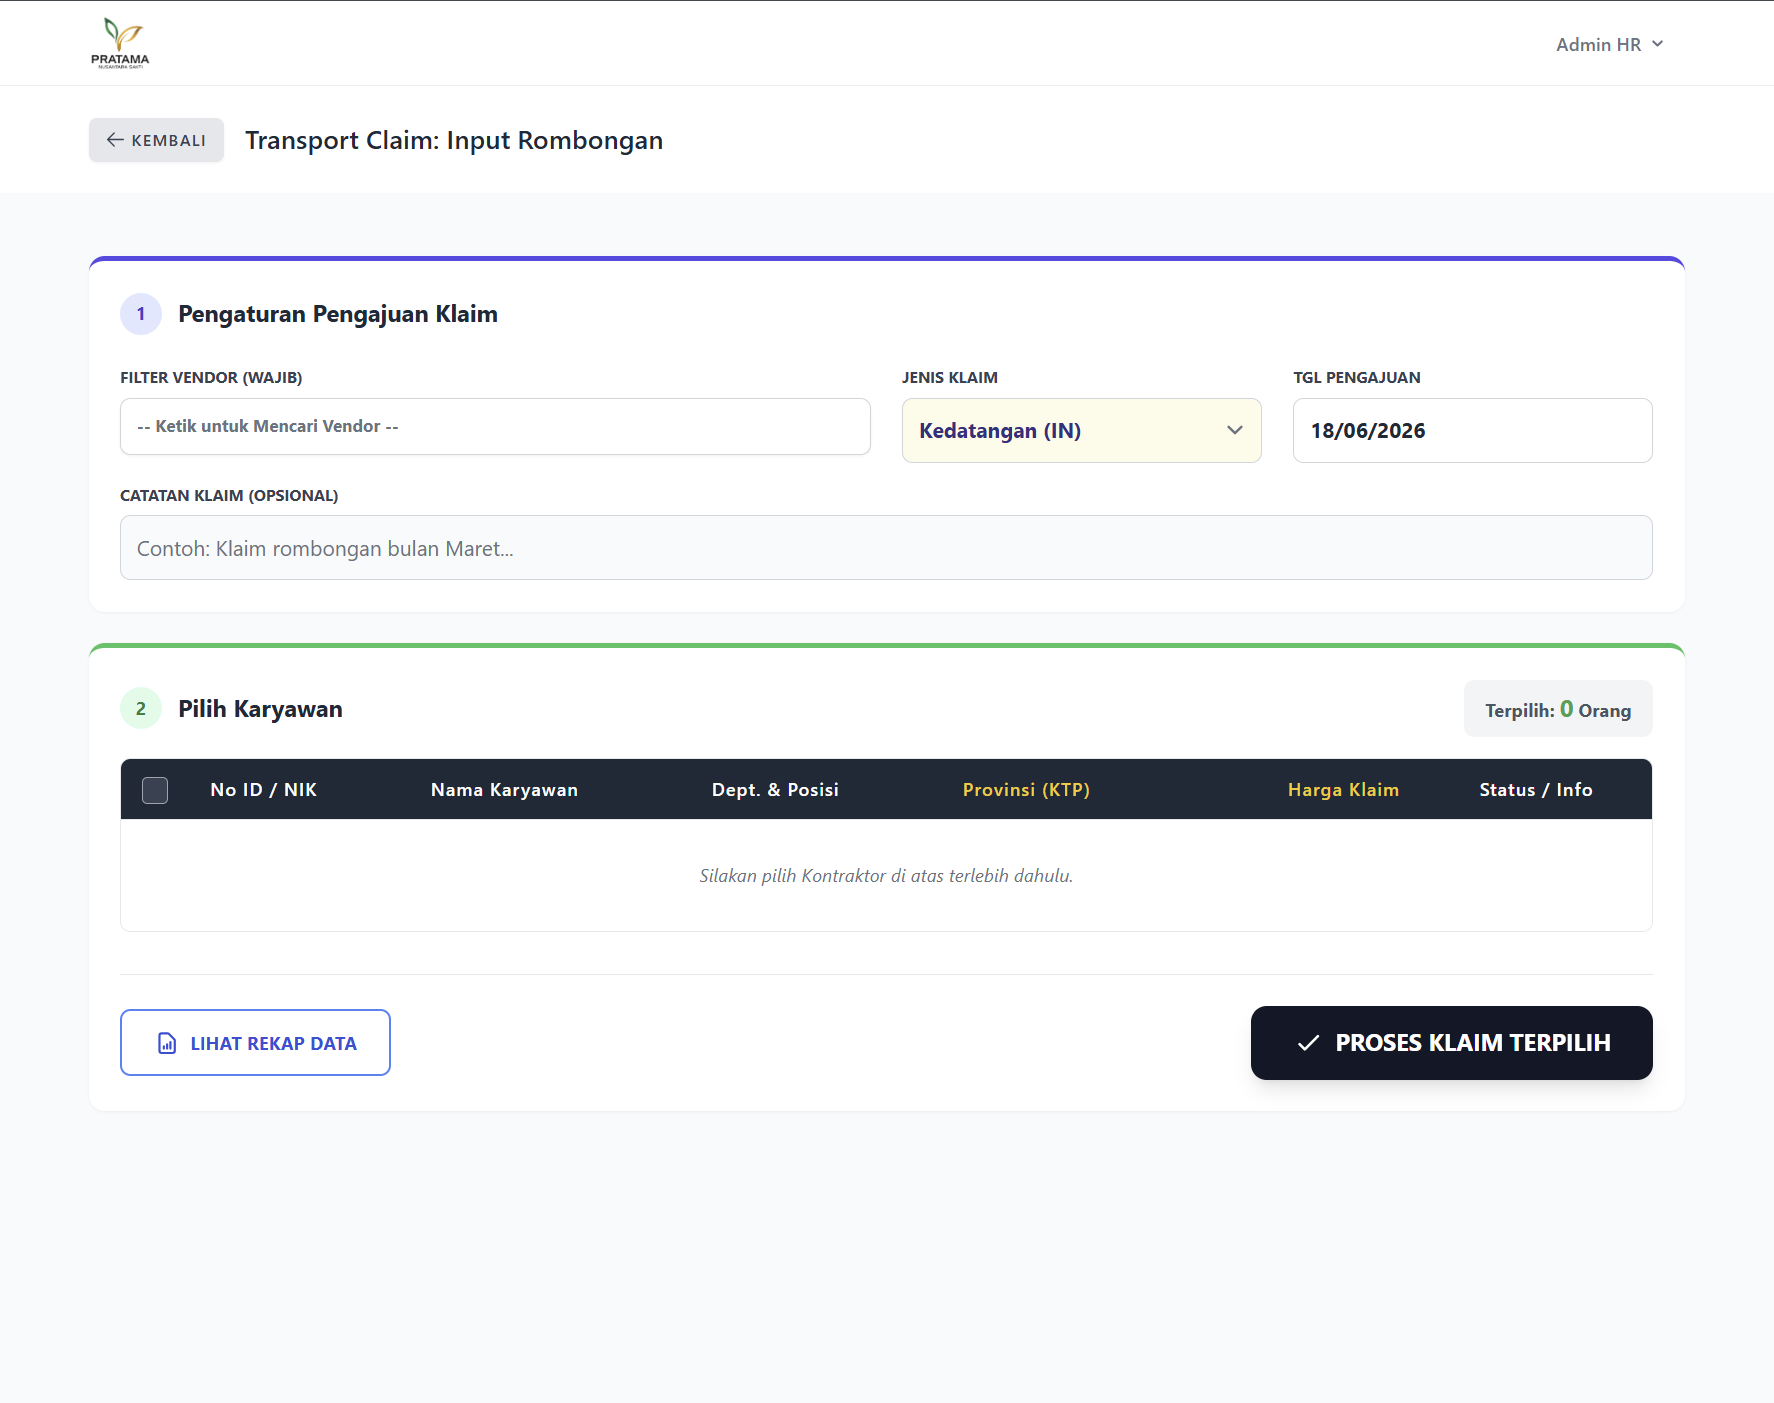
\includegraphics[width=0.9\textwidth]{assets/pics/Transport_Claim.png}}
    \caption{Antarmuka fitur Klaim Transport (\textit{Transport Claim})}
    \label{fig:ui-claim}
\end{figure}

% --- FITUR 3: SURAT IZIN KELUAR ---
\begin{figure}[H]
    \centering
    \frame{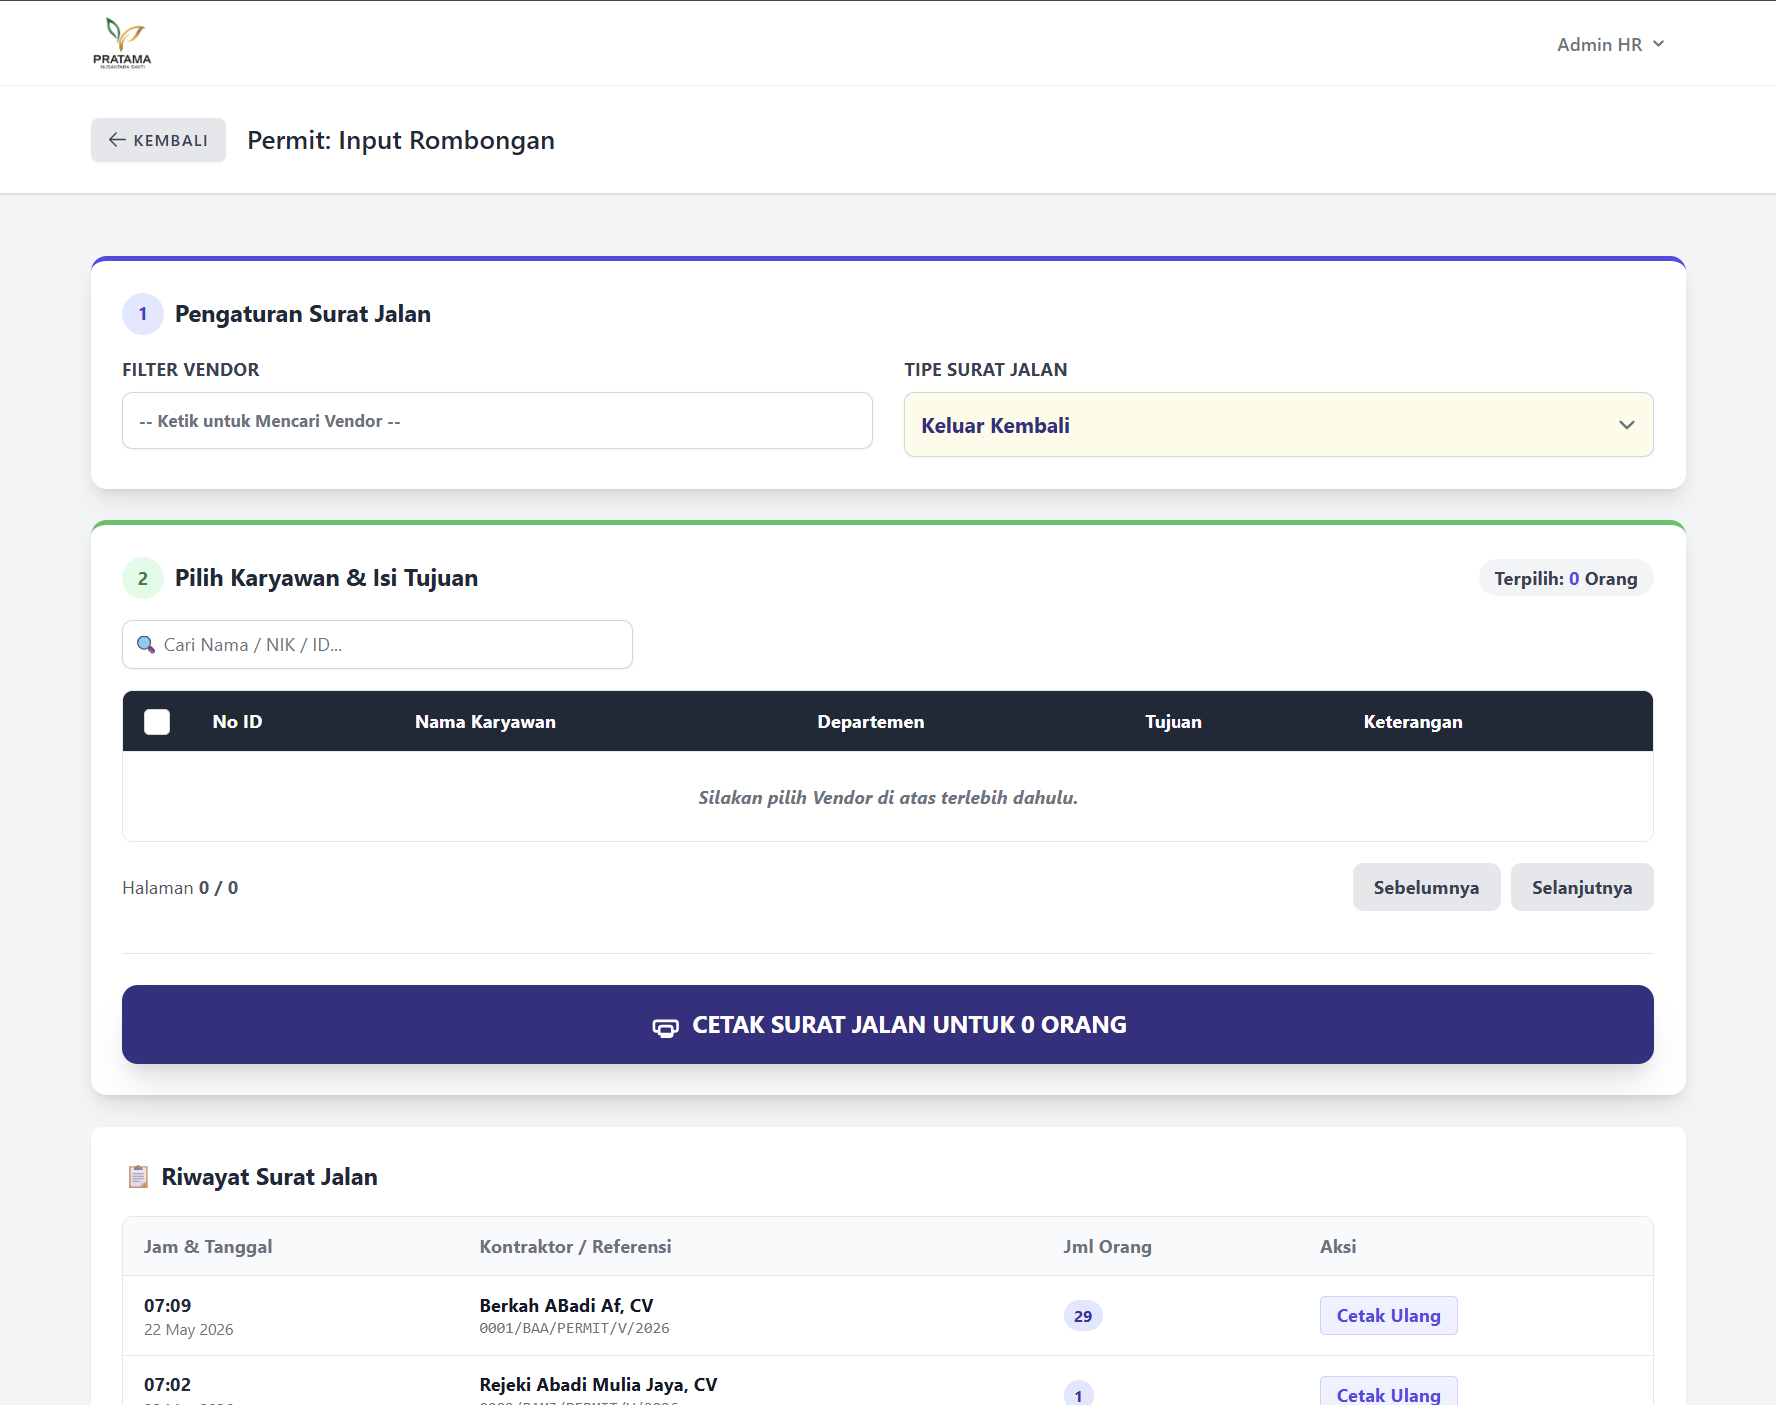
\includegraphics[width=0.9\textwidth]{assets/pics/Permit.png}}
    \caption{Antarmuka fitur Surat Izin Keluar (\textit{Exit Permits})}
    \label{fig:ui-permit}
\end{figure}
\clearpage

% --- FITUR 4: MANAJEMEN TARIF TRANSPORT ---
\begin{figure}[H]
    \centering
    \frame{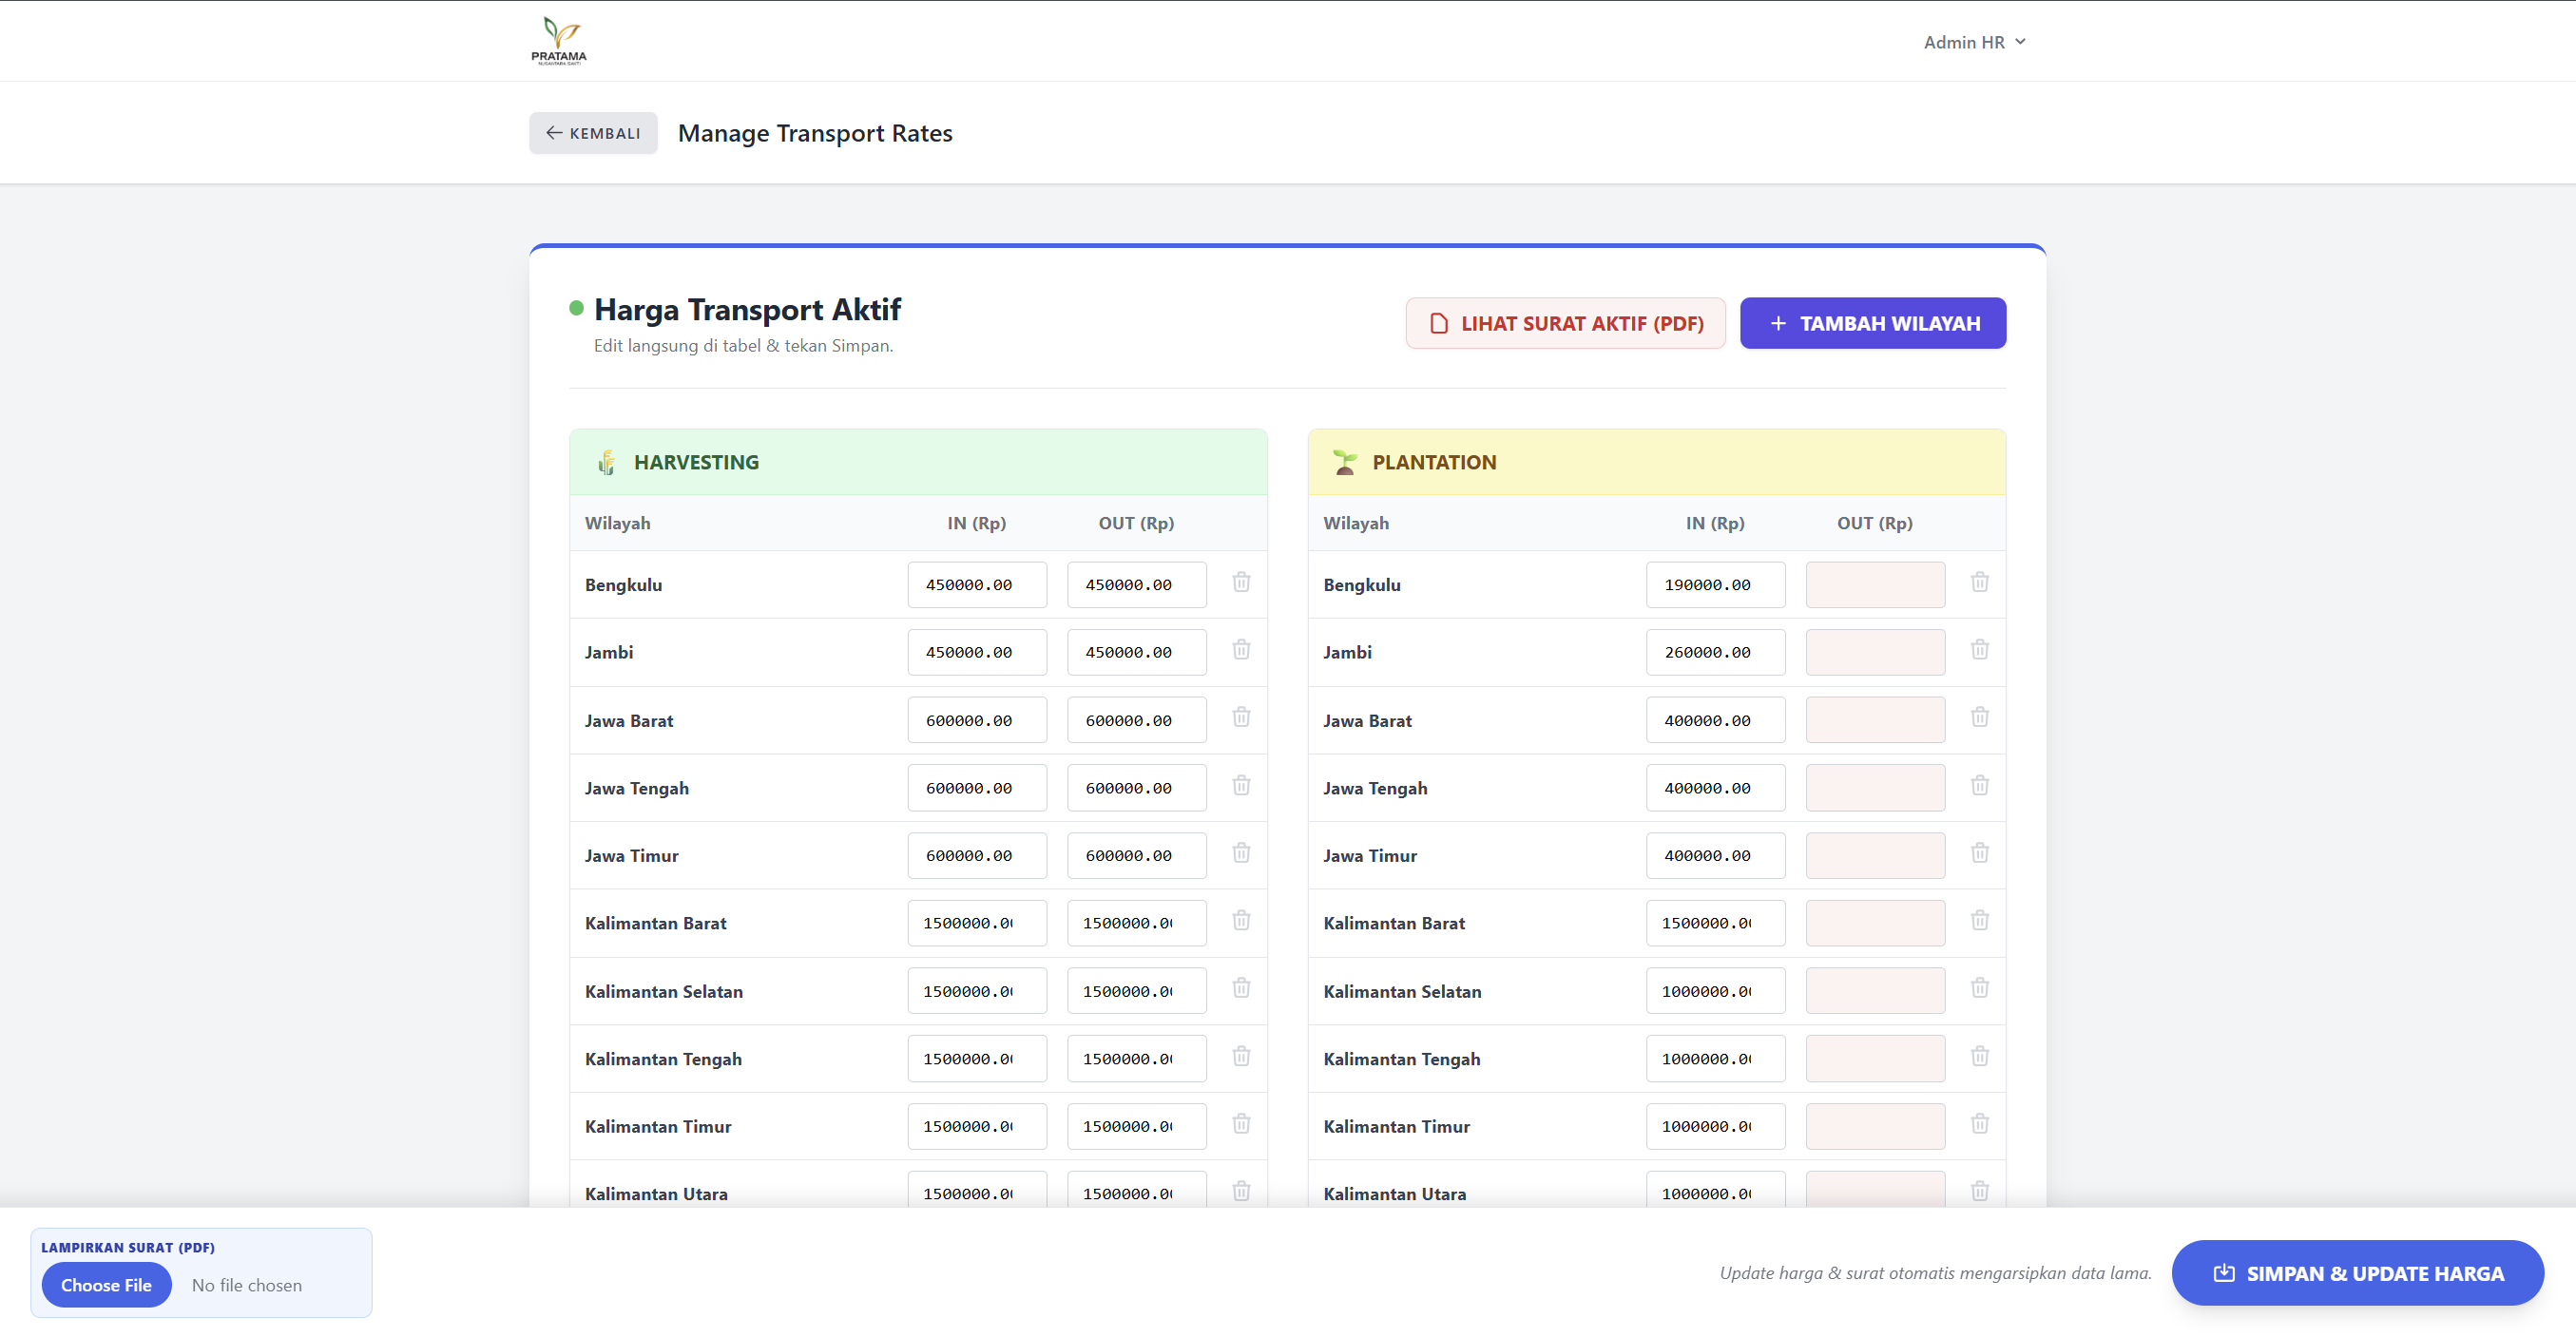
\includegraphics[width=\textwidth]{assets/pics/Manage_Rates.png}}
    \caption{Antarmuka fitur Manajemen Tarif Transport (\textit{Manage Rates})}
    \label{fig:ui-rates}
\end{figure}

% --- FITUR 5: PERSETUJUAN KARYAWAN ---
\begin{figure}[H]
    \centering
    \frame{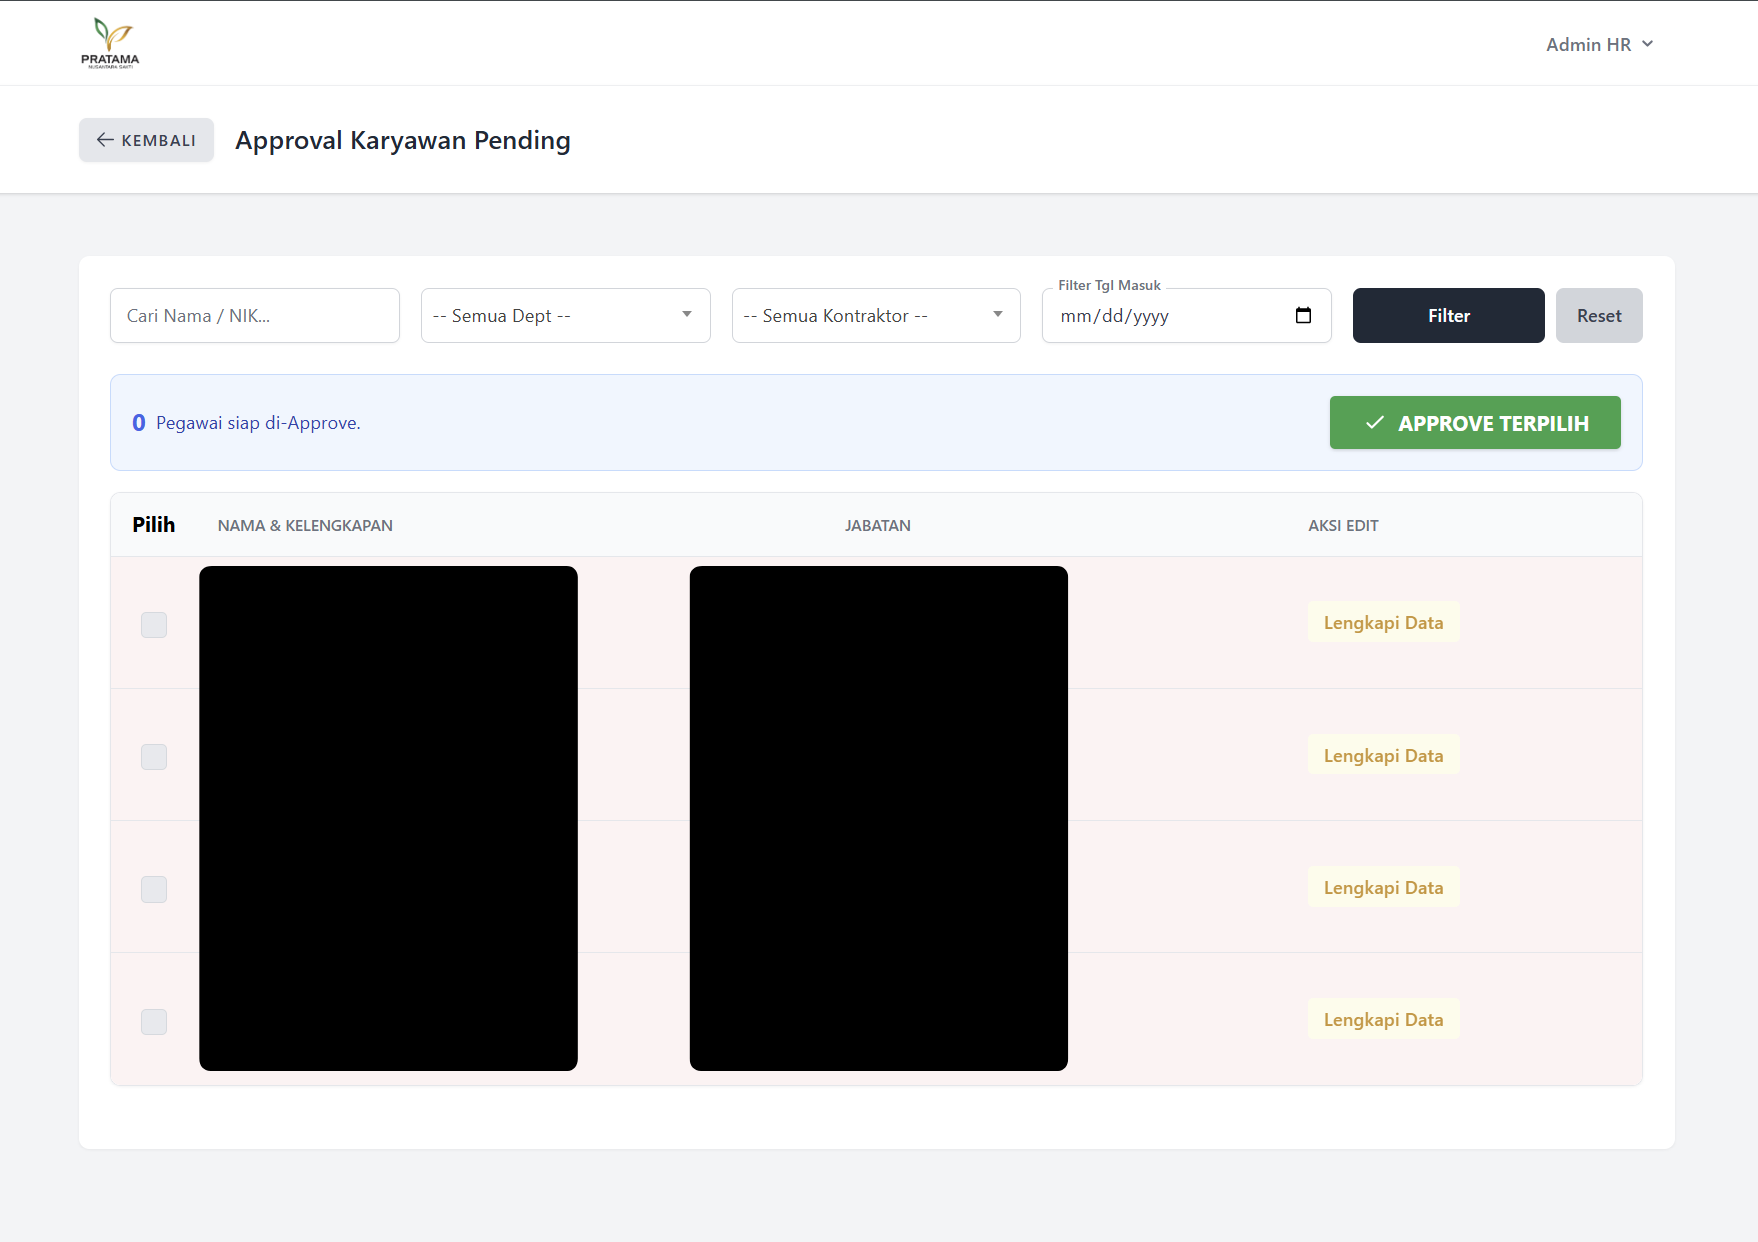
\includegraphics[width=0.9\textwidth]{assets/pics/User_Approval.png}}
    \caption{Antarmuka fitur Persetujuan Karyawan (\textit{Employees Approval})}
    \label{fig:ui-approval}
\end{figure}
\clearpage

% --- FITUR 6: MANAJEMEN PENGGUNA ---
\begin{figure}[H]
    \centering
    \frame{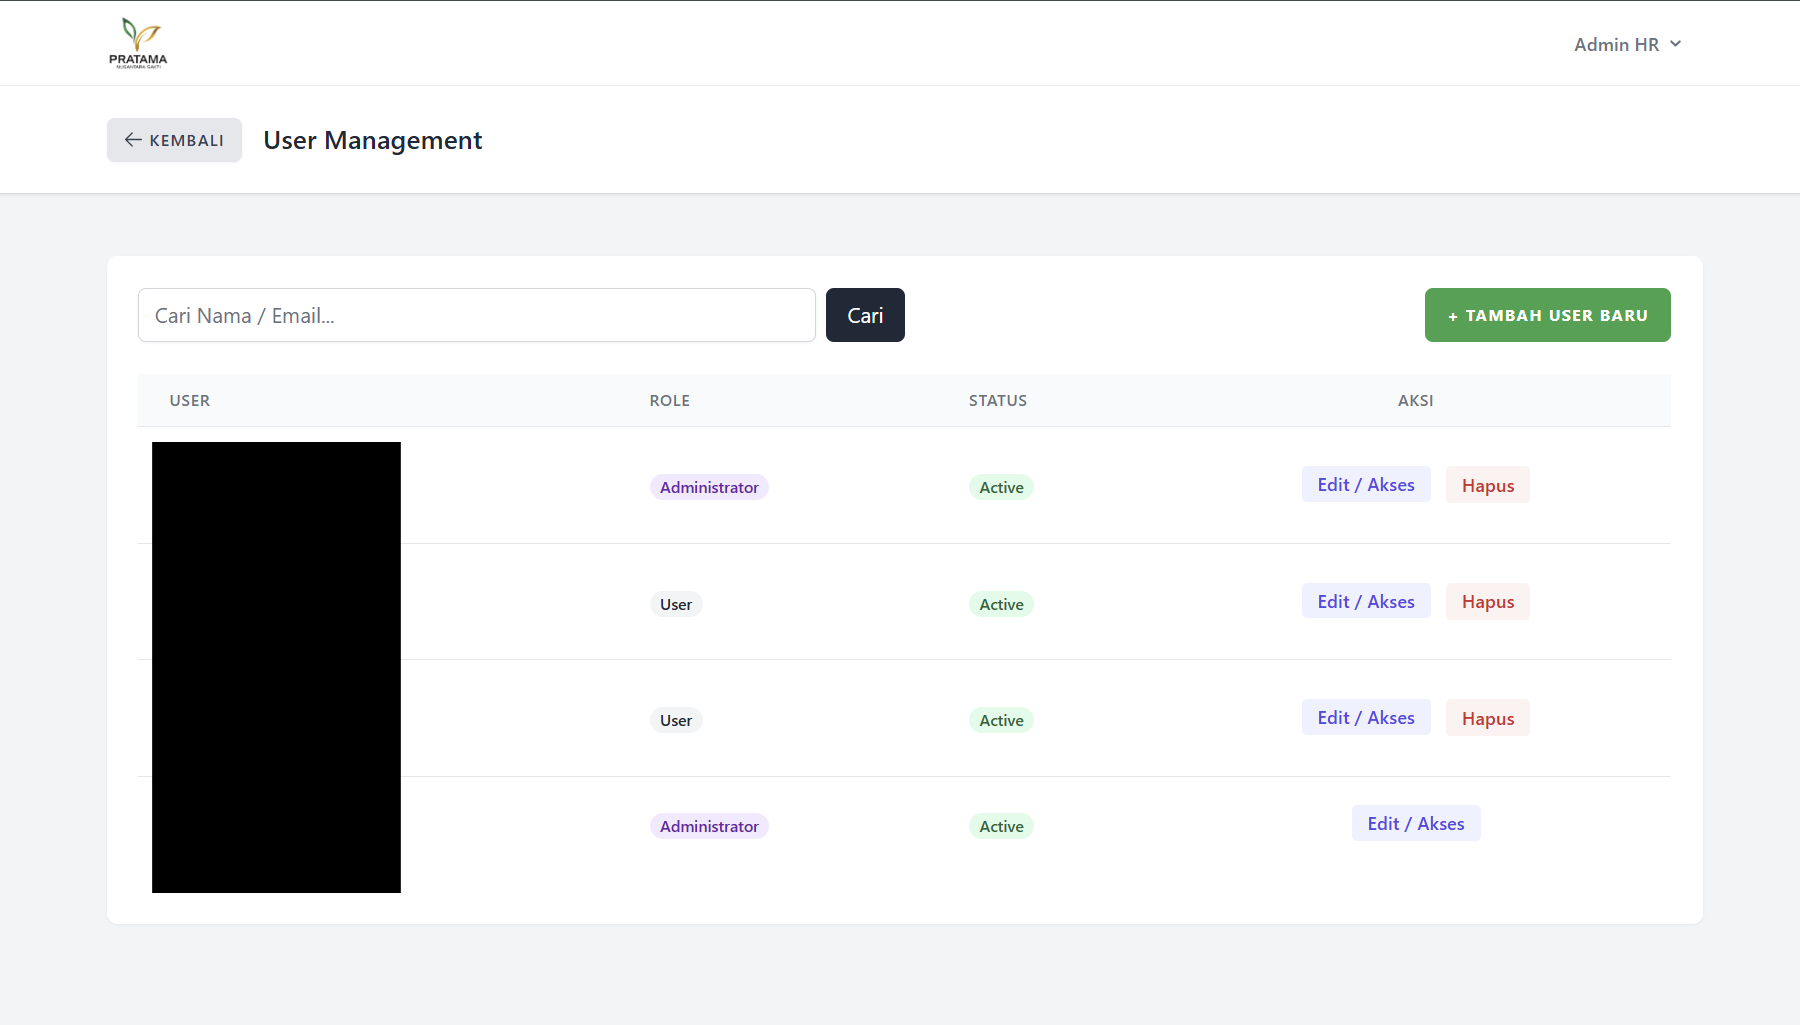
\includegraphics[width=0.9\textwidth]{assets/pics/User_Management.png}}
    \caption{Halaman daftar pengguna pada fitur Manajemen Pengguna (\textit{User Management})}
    \label{fig:ui-usermgmt}
\end{figure}

\begin{figure}[H]
    \centering
    \frame{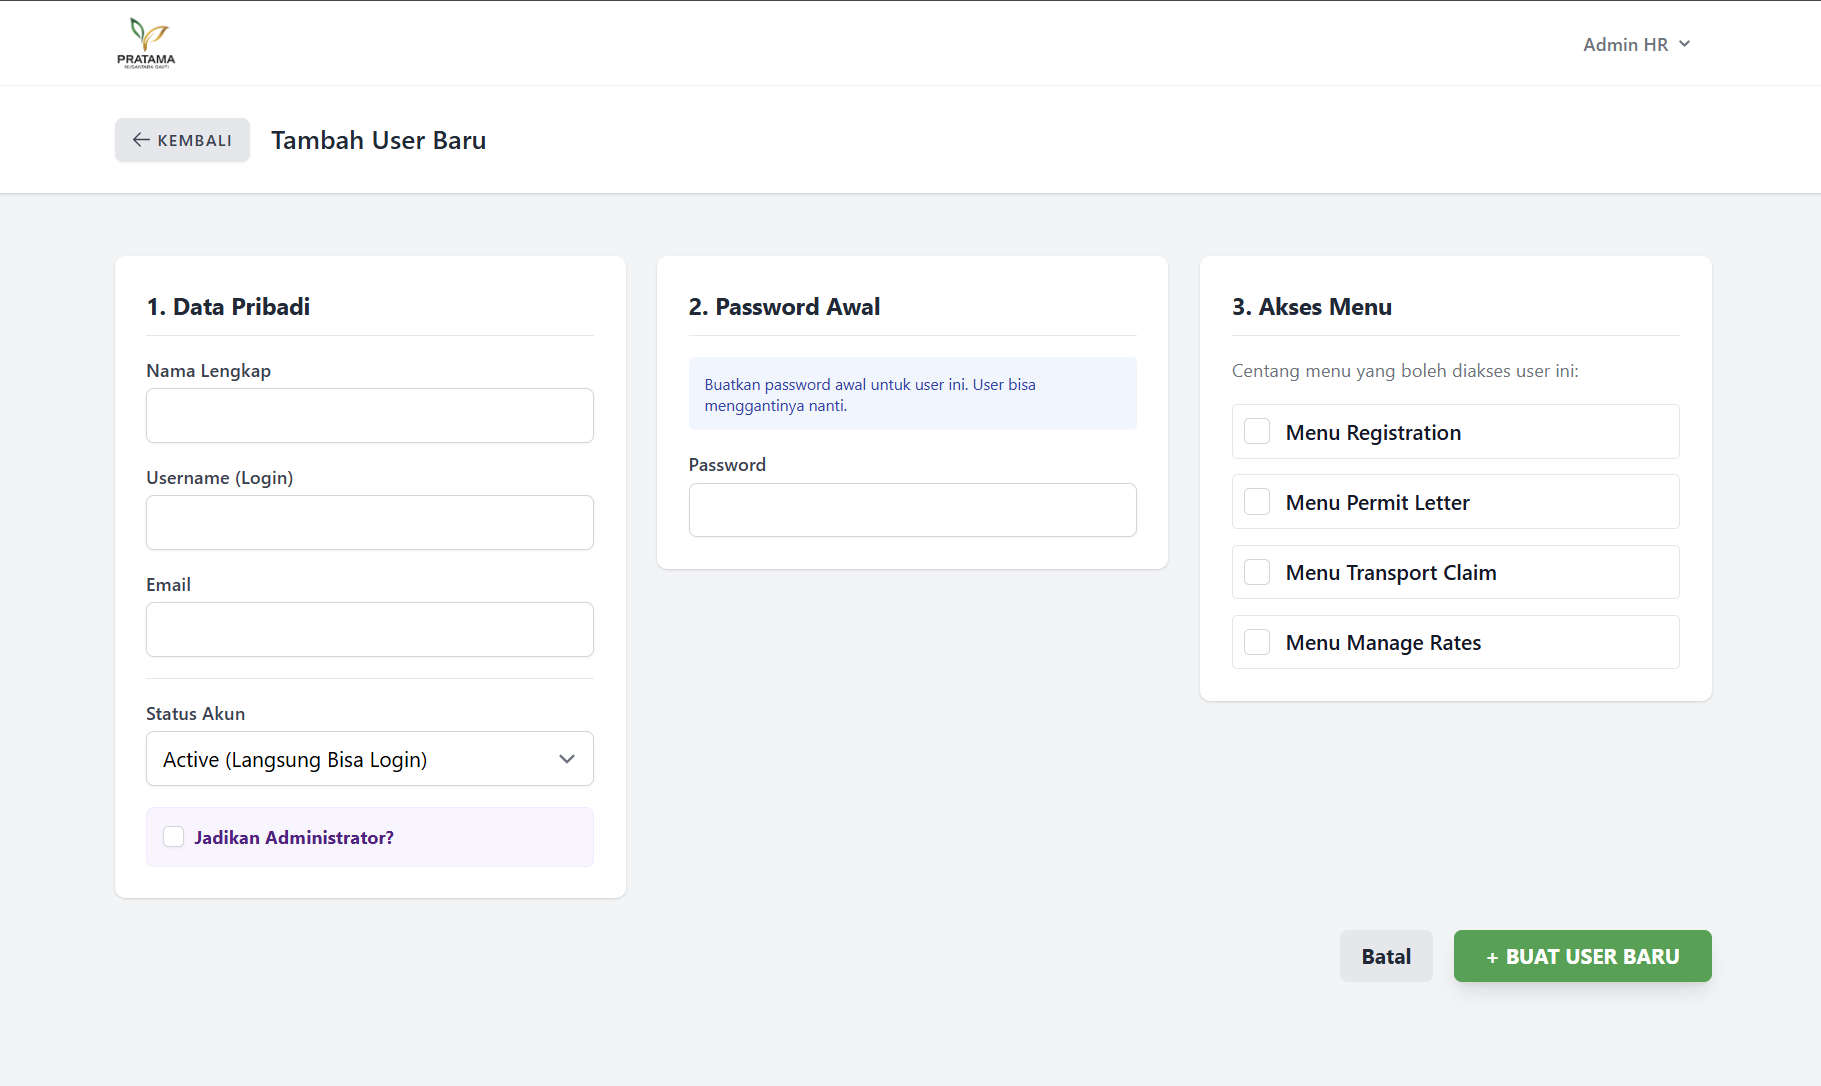
\includegraphics[width=0.9\textwidth]{assets/pics/Add_User.png}}
    \caption{Formulir penambahan pengguna baru beserta pengaturan hak akses menu (RBAC)}
    \label{fig:ui-tambah-user}
\end{figure}
\clearpage

% --- DASHBOARD ANALYTICS ---
\begin{figure}[H]
    \centering
    \frame{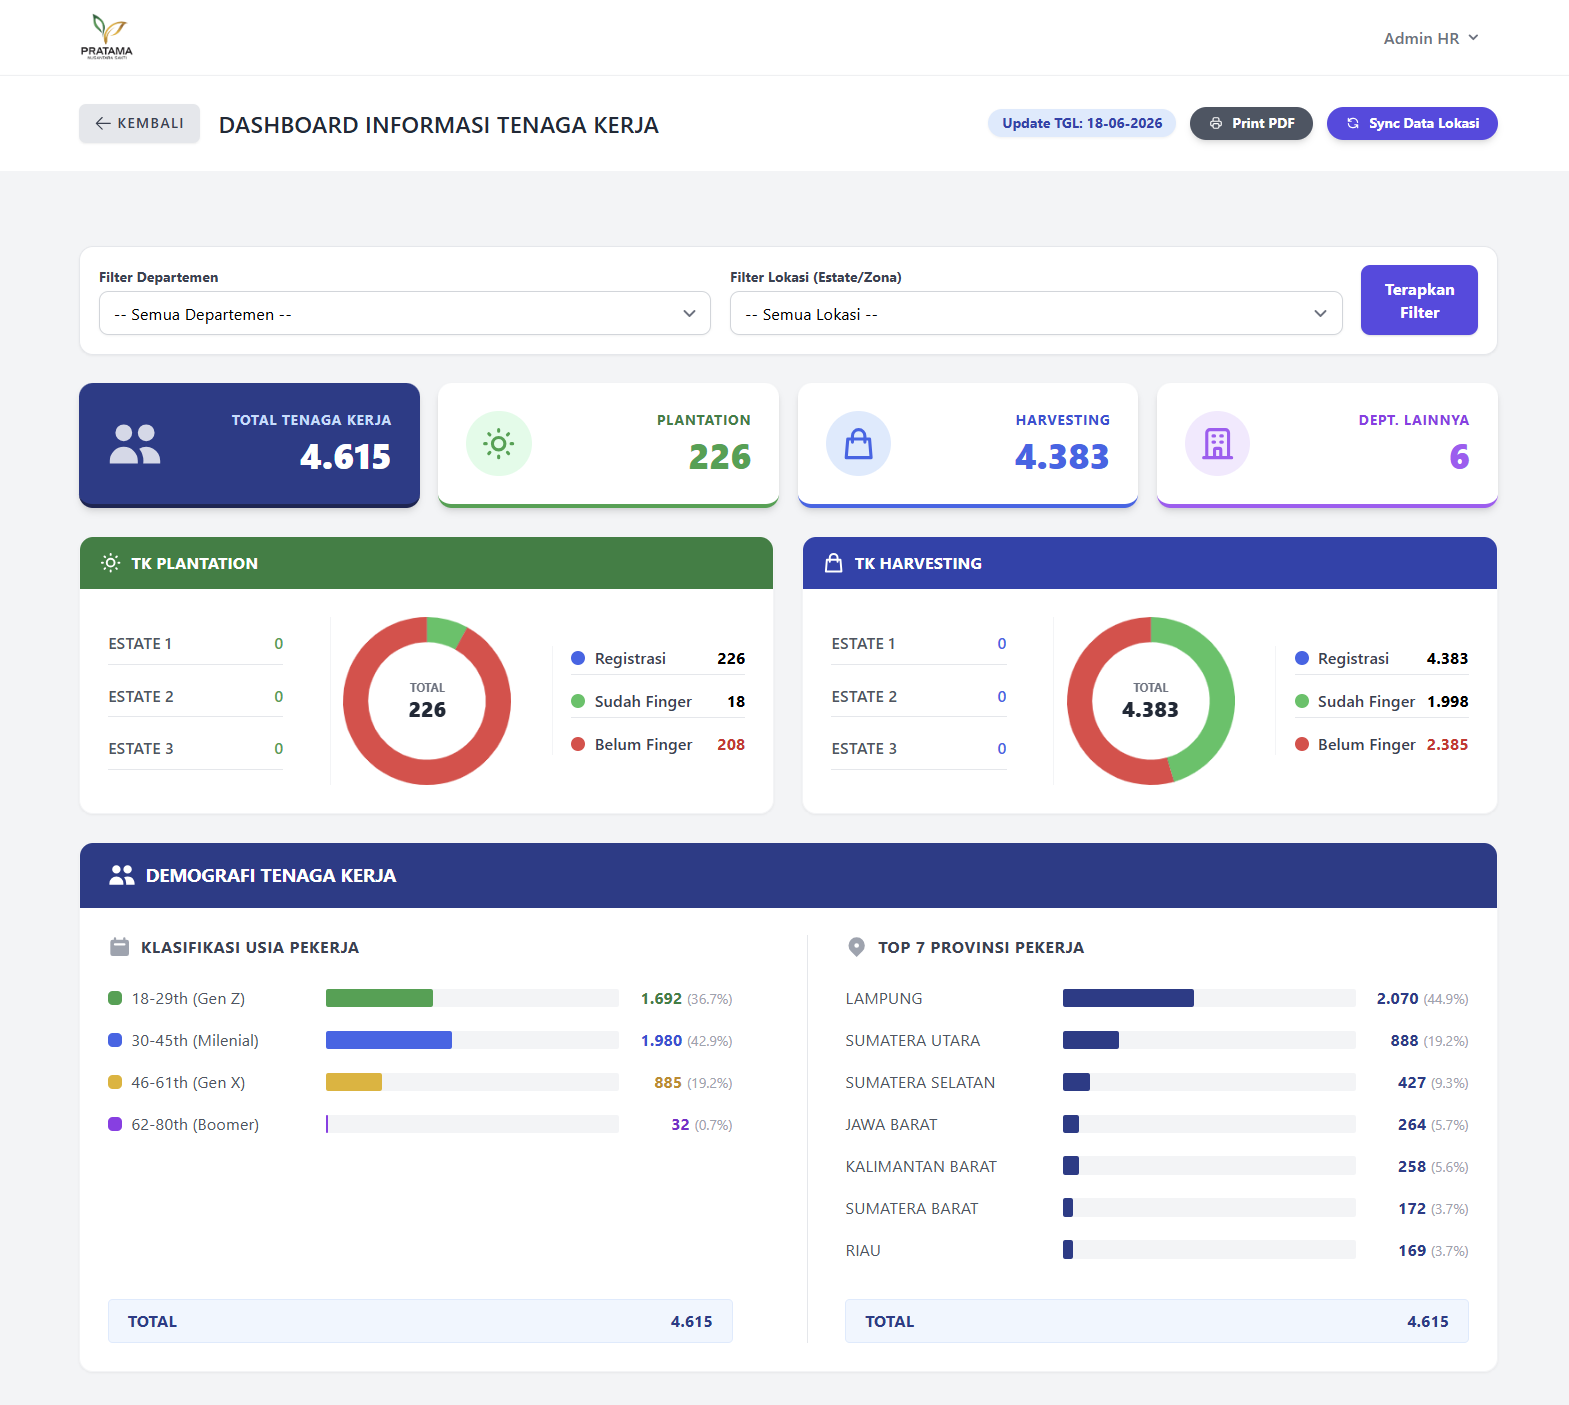
\includegraphics[width=0.9\textwidth]{assets/pics/Dashboard_Analytics.png}}
    \caption{Dashboard Informasi Tenaga Kerja yang menyajikan ringkasan data secara visual}
    \label{fig:ui-dashboard}
\end{figure}
\clearpage



